%%%%%%%%%%%%%%%%%%%%%%% file template.tex %%%%%%%%%%%%%%%%%%%%%%%%%
%
% This is a general template file for the LaTeX package SVJour3
% for Springer journals.          Springer Heidelberg 2010/09/16
%
% Copy it to a new file with a new name and use it as the basis
% for your article. Delete % signs as needed.
%
% This template includes a few options for different layouts and
% content for various journals. Please consult a previous issue of
% your journal as needed.
%
%%%%%%%%%%%%%%%%%%%%%%%%%%%%%%%%%%%%%%%%%%%%%%%%%%%%%%%%%%%%%%%%%%%
%
% First comes an example EPS file -- just ignore it and
% proceed on the \documentclass line
% your LaTeX will extract the file if required
\begin{filecontents*}{example.eps}
%!PS-Adobe-3.0 EPSF-3.0
%%BoundingBox: 19 19 221 221
%%CreationDate: Mon Sep 29 1997
%%Creator: programmed by hand (JK)
%%EndComments
gsave
newpath
  20 20 moveto
  20 220 lineto
  220 220 lineto
  220 20 lineto
closepath
2 setlinewidth
gsave
  .4 setgray fill
grestore
stroke
grestore
\end{filecontents*}
%
\RequirePackage{fix-cm}
%
%\documentclass{svjour3}                     % onecolumn (standard format)
\documentclass[smallcondensed]{svjour3}     % onecolumn (ditto)
%\documentclass[smallextended]{svjour3}       % onecolumn (second format)
%\documentclass[twocolumn]{svjour3}          % twocolumn
%
\smartqed  % flush right qed marks, e.g. at end of proof
%
\usepackage{graphicx}
%
% \usepackage{mathptmx}      % use Times fonts if available on your TeX system
%
% insert here the call for the packages your document requires
\usepackage{geometry,enumerate,datetime}                
\usepackage{graphicx}
\usepackage{amssymb,amsmath}
\usepackage{epstopdf}
\usepackage{array}
\usepackage{subfigure}
\usepackage{tensor,color}
\usepackage{tikz,pgfplots}
%\usepackage{latexsym}
% etc.
%
% please place your own definitions here and don't use \def but
\newcommand{\todo}[1]{ \fbox{{\bf TODO:} \color{red} #1}}
\newcommand{\lap}{\bigtriangleup}
\newcommand{\C}{C_k}
\renewcommand{\S} {\mathcal{S}}
\newcommand{\bigO} {\mathcal{O}}
\newcommand{\p}{\partial}
\newcommand{\e}{\varepsilon}
\newcommand{\s}{\ss}
\newcommand{\R}{I \! \! R^3}
\renewcommand{\H}{\mathcal{H}}
\newcommand{\pderiv}[2]{\frac{\partial #1}{\partial #2}}
% \newcommand{}{}
%
% Insert the name of "your journal" with
 \journalname{Advances in Computational Mathematics}
%
\begin{document}


\title{Integral equation methods for the Yukawa-Beltrami equation on
the sphere 
}


%\date{$^1$Department of Mathematics, Simon Fraser University, \\[1mm]
%$^2$Institute for Computational Engineering and Sciences, University of
%Texas at Austin, \\[1mm]
%$\clubsuit$ {\small \tt mkropinksi@math.sfu.ca} \quad
%$\diamondsuit$ {\small \tt nigam@math.sfu.ca}\\
%$\spadesuit$ {\small \tt quaife@ices.utexas.edu}}

%\titlerunning{Short form of title}        % if too long for running head

\author{M.C.~Kropinski    \and
        N.~Nigam          \and
        B.~Quaife}

\authorrunning{Kropinski, Nigam, Quaife} % if too long for running head

\institute{M.C.~Kropinski \at
              Department of Mathematics, Simon Fraser University \\
              \email{mkropins@math.sfu.ca}           %  \\
           \and
           N.~Nigam \at
              Department of Mathematics, Simon Fraser University \\
              \email{nigam@math.sfu.ca}           %  \\
          \and
          B.~Quaife \at 
              Institute for Computational Engineering and Science,
              University of Texas \\
              Tel.: +1-512-232-3509 \\
              Fax: +1-512-471-8694 \\
              \email{quaife@ices.utexas.edu}
}


\date{Received: date / Accepted: date}
% The correct dates will be entered by the editor


\maketitle

\begin{abstract}
An integral equation method for solving the Yukawa-Beltrami equation on
a multiply-connected sub-manifold of the unit sphere is presented. A
fundamental solution for the Yukawa-Beltrami operator is constructed.
This fundamental solution can be represented by conical functions.
Using a suitable representation formula, a Fredholm equation of the
second kind with a compact integral operator needs to be solved.  The
discretization of this integral equation leads to a linear system whose
condition number is bounded independent of the size of the system.
Several numerical examples exploring the properties of this integral
equation are presented. 
\keywords{Yukawa-Beltrami boundary value problems \and Integral equations}
% \PACS{PACS code1 \and PACS code2 \and more}
 \subclass{35J25 \and 45B05}
\end{abstract}


%%%%%%%%%%%%%%%%%%%%%%%%%%%%%%%%%%%%%%%%%%%%%%%%%%%%%%%%%%%%%%%%%%%%%%%%
\section{Introduction}

Applications of partial differential equations (PDEs) on surfaces and
manifolds include image processing, biology, oceanography, and fluid
dynamics~\cite{Chaplain,Myers,Witkin}.  Since solutions of these PDEs
depend both on local {\it and} global properties of a given
differential operator on the manifold, standard numerical
discretization methods developed for PDEs in the plane or in
$\mathbb{R}^3$ need to be modified. Recent work in this direction
includes the closest point method~\cite{ruuth}, surface
parametrization~\cite{floater}, embedding functions,~\cite{Bertalmio},
and projections onto an approximation of the manifolds by tessellations
of simpler, non-curved domains (such as triangles)~\cite{lindblom}. 

It is well-known that for elliptic PDEs in $\mathbb{R}^2$ or
$\mathbb{R}^3$, numerical methods based on integral equation
formulations can offer significant advantages: efficiency is achieved
through dimension reduction, and superior stability of such methods
allows highly accurate solutions to be computed.  In addition, the
development of efficient numerical techniques such as the fast
multipole method or fast direct solvers have made integral equation
approaches significantly faster than many other currently available
schemes.  Relatively little work has been done, however, on using
integral equation methods for numerically investigating elliptic PDEs
on subsurfaces of manifolds.  Some prior work in this direction for the
Laplace-Beltrami operator on the surface $\cal{S}$ of the unit sphere
was presented in~\cite{gemmrich,kro:nig2013}.

In this paper we present a reformulation of a boundary value problem
for the Yukawa-Beltrami equation on the surface of the unit sphere
$\S$  in terms of boundary integral equations. Concretely, let $\Omega$
denote a sub-manifold of $\S$, and let $\Gamma$ denote its boundary. By
this we mean that $\Gamma$ is a closed curve  on $\S$ which divides
$\S$ into two (not necessarily connected) parts $\Omega$ and
$\Omega^{c}$. In particular, $\Gamma = \partial\Omega$ is the boundary
curve of $\Omega$. We wish to solve the Yukawa boundary value problem:
\begin{subequations}
\label{bigmodel}
  \begin{align}
    -\lap_\S u(x)+k^2  u(x)&= f({ x}), && \mbox{for} \: x \in \Omega, \\
    u(x)&=g(x), &&\mbox{for} \; x \in \Gamma. 
  \end{align}
\end{subequations}
Here $\lap_{\S}$ is the Laplace-Beltrami operator on $\S$ and $k>0 \in
\mathbb{R}$ is constant. This  problem arises in the context of solving
the isotropic heat equation via Rothe's method.  By first applying a
semi-implicit time discretization to the heat equation, time-stepping
then involves repeatedly solving an elliptic PDE of the
form~\eqref{bigmodel}, where $k^2 = O(1/\Delta t)$.  In fact, this
strategy is not restricted to the heat equation since the
PDE~\eqref{bigmodel} also arises when an IMEX
method~\cite{asc:ruu:wet1995} is applied to PDEs that involve the heat
operator.  Therefore, possible applications span many fields of science
such as fluid dynamics.  This approach is discussed in~\cite{rothe:heat}
for several PDEs in the plane.

We recall that the exterior boundary value problem for the Yukawa
operator $(-\lap + k^2)$  in $\mathbb{R}^2$ is well-posed if we seek
$H^1$ (weak) solutions, even without the specification of a radiation
condition (see, e.g.,~\cite{gatica}). This is in contrast to the
exterior problem for the Laplacian.  In~\cite{gemmrich}, it was observed
that the single-layer operator for the Laplace-Beltrami did not satisfy
the associated boundary value problem on $\S$ unless a further
constraint was satisfied. Experience with the Yukawa operator in
$\mathbb{R}^2$~\cite{kro:qua2011,qua2011} suggests that any issues
concerning unique solvability which arise for the Laplace-Beltrami
operator when we move to a compact manifold will be ameliorated for the
Yukawa-Beltrami operator.  We shall see this is indeed the case. In
fact, when $k>\frac{1}{2}$, using conical functions, it can be readily
seen that the single-layer potential exactly solves the boundary value
problem.  (In case we solve the Yukawa-Beltrami problem on a sphere of
radius $R$, we require $kR>1/2$.)

To simplify the exposition and analysis, we shall concentrate on
locating the homogeneous solution of~\eqref{bigmodel}.  In other words:
{\it Find a smooth $u$ such that for given smooth Dirichlet data $g$}
\begin{subequations}
  \label{DBVP}
  \begin{align}
    -\lap_{\S} u(x) +k^2u(x)\, &= \, 0, &&\mbox{for} \; 
      x \in { \Omega},\\
    u(x) &= g(x), &&\mbox{for} \; x \in \Gamma.
  \end{align}
\end{subequations}
We note that we could equivalently have chosen to study the Neumann or
Robin problem for the system.  We wish to solve~\eqref{DBVP} by
reformulating this boundary value problem as an integral equation. As is
expected, the process of reformulation is not unique; we shall be
employing a layer ansatz based on a parametrix for the Yukawa-Beltrami
operator, and solving an integral equation for an unknown density.  The
choice of parametrix is not unique, and we derive a particularly
convenient parametrix involving conical functions. By proceeding with a
double-layer ansatz based on this parametrix, a well-conditioned
Fredholm equation of the second kind results. Several numerical examples
are presented which illustrate the analytic properties of this integral
equation.


%%%%%%%%%%%%%%%%%%%%%%%%%%%%%%%%%%%%%%%%%%%%%%%%%%%%%%%%%%%%%%%%%%%%%%%%
\subsection{Some preliminaries}
We favour an intrinsic definition, and where possible identify $x\in \S$
by two independent variables (the spherical angles), $x=x(\phi,\theta)$.
We can also describe this point in terms of a Euclidean coordinate
system in $\mathbb{R}^3$ whose origin is at the center of mass of the
sphere: 
\begin{align*}
 x= x(\varphi,\theta) \, \equiv \, \left( 
  \begin{array}{c}
    \cos \varphi \sin \theta \\
    \sin \varphi \sin \theta \\
    \cos \theta
  \end{array} 
  \right) \in{\S}, \quad \varphi \in [0,2\pi), 
    \quad \theta \in [0,\pi].
\end{align*}
We also recall that on $\S$, the Laplace-Beltrami operator  $\lap_\S$
is defined as
\begin{align*}
  \lap_S u(x) \, = \, \left[
  \frac{1}{\sin^2 \theta} \frac{\partial^2}{\partial \varphi^2} +
  \frac{1}{\sin \theta} \frac{\partial}{\partial \theta}
  \left(\sin \theta \frac{\partial}{ \partial \theta}\right)
  \right] u(x(\varphi,\theta)).
\end{align*}

If two points $x,y$ lie on the unit sphere, with spherical coordinates
$x=x(\phi,\theta)$ and $y=(\alpha,\beta)$, then we describe the solid
angle between them (a measure of their distance in the metric on $\S$)
by
\begin{align*}
  <x,y> =\cos(\phi-\alpha)\sin(\theta)\sin(\beta)+
    \cos(\theta)\cos(\beta).
\end{align*} 
In particular if $y$ is the North Pole then  $\beta=0$ and
$<x,y>=\cos(\theta)$. (If we denoted $x,y$  by their Cartesian
coordinates $(x_1,x_2,x_2),(y_1,y_2,y_3)$, then $<x,y> = \sum_{i=1}^3
x_iy_i$.) The distance between $x$ and $y$ in the 3-dimensional
Euclidean metric $\|x-y\|$ is given by 
\begin{align*}
  \|x-y\|^2 := 2-2<x,y>, \qquad \Rightarrow \qquad 
    <x,y>= 1-\frac{\|x-y\|^2}{2}.
\end{align*}

We remind the reader of some useful vectorial identities on the sphere.
Let $ \vec{e}_\theta, \vec{e}_{\varphi} $ be the usual unit vectors in
spherical coordinates.  Recall that we can define the surface gradient
of a scalar $f$ on $\S$ as
\begin{align*}
  \nabla_{\S} f(x) \,  = \, \frac{1}{\sin \theta}
  \frac{\partial f}{\partial \varphi} \,\vec{e}_{\varphi} + 
  \frac{\partial f}{\partial \theta}\, \vec{e}_{\theta}.
\end{align*}
In the same way, the surface divergence for a vector-valued
function $\vec{V}$ on the sphere can be written as
\begin{align*}
  \mbox{div}_{\S} \vec{V}(x) \, = \, 
  \frac{1}{\sin \theta} \left(
  \frac{\partial}{\partial \varphi}
  V_{\varphi}(\varphi,\theta) +
  \frac{\partial}{\partial \theta} ((\sin\theta) \, 
  V_{\theta}(\varphi,\theta) ) \right).
\end{align*}
We easily see the identity $\lap_{\S}u(x) \, = \,
\mbox{div}_{\S}\nabla_{\S} u(x)$.  The vectorial surface rotation for a
scalar field $f$ on the sphere is 
\begin{align*}
  \underline{\mbox{curl}}_{\S} f(x) \, = -\, 
  \frac{\partial f}{\partial \theta} \,\vec{e}_{\varphi} + 
  \frac{1}{\sin\theta}\frac{\partial f}{\partial \varphi}\, 
  \vec{e}_{\theta},
\end{align*}
and the (scalar) surface rotation of a vector field $\vec{V}$ is
\begin{align*}
  \mbox{curl}_{\S} \vec{V}(x) \, = \,
  \frac{1}{\sin \theta} \left(
  - \frac{\partial}{\partial \varphi} V_{\theta}(\varphi,\theta) +
  \frac{\partial}{\partial \theta} ((\sin \theta) \,   
  V_{\varphi}(\varphi,\theta)) \right).
\end{align*}
We then obtain another vectorial identity for the Laplace-Beltrami
operator:
\begin{align*}
  \lap_{\S} u(x) \, = \, - \mbox{curl}_{\S} 
  \underline{\mbox{curl}}_{\S} u(x) \quad \mbox{for} \; x \in {\S}.
\end{align*}


Stokes' theorem for the  smooth positively oriented curve $\Gamma$ and
the enclosed region $\Omega$ may be written  as
\begin{align*}
  \int\limits_{\Omega} \mbox{curl}_{\S} \vec{V}(x) d\sigma_x \, = \,
  \int\limits_\Gamma \vec{V}(x) \cdot \vec{t}(x) \, ds_x .
\end{align*}
Here, $\vec{t}$ is the unit tangent vector to $\Gamma$, $d\sigma$ is an
area element, and $ds$ is an arclength element. We note that a similar
identity holds for the region $\Omega^{c}$, with care taken with the
orientation of the tangent.  Now, setting $\vec{V} = v(x) \vec{W}(x)$
and applying the product rule we have
\begin{align*}
  \int\limits_{\Omega} \underline{\mbox{curl}}_{\S} v(x) \cdot
  \vec{W}(x) \, d\sigma_x \, = \, 
  -\int\limits_{\Gamma} v(x) [\vec{W}(x) \cdot \vec{t}(x)] ds_x +
  \int\limits_{\Omega} v(x) \mbox{curl}_{\S} \vec{W}(x) d\sigma_x .
\end{align*}
With $\vec{W}(x) = \underline{\mbox{curl}}_{\S} u(x)$ we finally
obtain Green's first formula for the Laplace-Beltrami operator
$\lap_{\S}$,
\begin{align}
  \label{Green1}
  -\int\limits_{\Omega} \underline{\mbox{curl}}_{\S} v(x) \cdot
  \underline{\mbox{curl}}_{\S} u(x) \, d\sigma_x 
  =& \int\limits_{\Gamma} v(x) [\underline{\mbox{curl}}_S u(x) \cdot 
  \mathbf{t}(x)] ds_x +\int\limits_{\Omega} v(x) \lap_{\S}u(x) d\sigma_x.
\end{align}

We obtain Green's second formula by interchanging the roles of $u$ and
$v$ in~\eqref{Green1}, subtracting the two identities, and using the
symmetry of the left hand side
\begin{align}
  &\int\limits_{\Omega} v(x)(-\lap_{\S}u(x) + k^2 u(x))-
  u(x)(-\lap_{\S}v(x) +k^2v(x))\, d\sigma_x \nonumber \\
  =&\int\limits_\Gamma [v(x)\,\underline{\mbox{curl}}_{\S} 
  u(x) - u(x)\, \underline{\mbox{curl}}_{\S}v(x)] \cdot 
  \vec{t}(x) ds_x.
  \label{Green2}
\end{align}

We shall make extensive use of these identities.


%%%%%%%%%%%%%%%%%%%%%%%%%%%%%%%%%%%%%%%%%%%%%%%%%%%%%%%%%%%%%%%%%%%%%%%%
\section{A fundamental solution and representation formula}
We seek a fundamental solution for the Yukawa-Beltrami operator
$(-\lap_\S + k^2)$.  Examining first the situation for the Yukawa
operator in the Euclidean plane, the fundamental solution of the Yukawa
operator, $(-\lap + k^2)$ in $\mathbb{R}^2$ is given by
$\frac{k^2}{2\pi} K_{0}(kr)$, where $r=\|\mathbf{x} - \mathbf{x}_{0}\|$
is the distance between the source and evaluation point in the
two-dimensional Euclidean metric. Here $K_{0}$ is the modified Bessel
function of order 0 which is analytic for non-zero argument, and has a
logarithmic singularity when the source and evaluation points coincide,
that is, when $r=0$.

On the surface of the sphere $\S$, we expect the fundamental solution
$G_k(x,x_{0})$ for the Yukawa-Beltrami operator to possess a
logarithmic singularity when $x$ approaches $x_{0}$. Exactly as was
done  with the Laplace-Beltrami operator in~\cite{gemmrich}, we could
define a parametrix for this operator by using the {\it distance
measured in the Euclidean norm in $\mathbb{R}^3$}. This would suggest
using $ \frac{k^2}{2\pi}K_0(k\|x-x_{0}\|)$.  Such a choice of
parametrix would be directly related to the fundamental solution of the
two-dimensional operator; the amount by which it fails to yield a dirac
measure is directly attributable to the difference between the
spherical and flat metrics.  In particular, with $r:=\|x-x_{0}\|$, we
have
\begin{align*}
  (-\lap_{\S} + k^{2})\frac{k^2}{2\pi}K_0(kr) = \delta(r) 
  +\frac{k^{4}r^{2}}{8\pi}K_{0}(kr) - \frac{k^{3}r}{4\pi}K_{1}(kr).
\end{align*}

While this is a perfectly reasonable parametrix, it is inconvenient
from the perspective of rewriting the Yukawa-Beltrami boundary value
problem in terms of a boundary integral equation. The term
$\frac{k^{4}r^{2}}{8\pi}K_{0}(kr) - \frac{k^{3}r}{4\pi}K_{1}(kr)$ will
result in {\it volumetric} constraints  appearing in an integral
equation representation. Such a term encapsulates the fact that we are
on a compact manifold, no longer on $\mathbb{R}^2$. Recall that for the
Laplace-Beltrami case, when $k=0$, this term
$\frac{k^{4}r^{2}}{8\pi}K_{0}(kr) - \frac{k^{3}r}{4\pi}K_{1}(kr)$
reduces to a constant; it is then possible to use a double-layer ansatz
in which no volumetric terms or constraints appear~\cite{kro:nig2013}.  

To avoid such complications, we shall instead derive a more convenient
parametrix.  In particular, we use the fundamental solution of the
Yukawa-Beltrami equation.  Without loss of generality we first set
$x_{0}$ to be the point at the north pole.  Let $x$ be some other point
on the sphere. The fundamental solution $G_k(x,x_0)$ depends on
$r_0(\theta)=\|x-x_0\|=\sqrt{2-2\cos(\theta)}$. Since there is no
angular dependence in $\phi$, the Yukawa-Beltrami operator reduces to
the second order ODE operator
\begin{align*}
  \mathcal{D}_k(u) := \frac{1}{\sin(\theta)}
  \frac{d}{d\theta}\left(\sin(\theta)
  \frac{d}{d\theta}u(r_0(\theta))\right)-k^2 u(r_{0}(\theta)).
\end{align*}
A simple change of variables allows us to rewrite $\mathcal{D}_k (u)=0$
as 
\begin{align}
  (1-z^2)\,w'' -2zw' + \left[\nu(\nu+1)\right]\,w = 0,
  \label{LegendrePequation}
\end{align}
where $\nu = \nu(k)$ satisfies $\nu(\nu + 1) = -k^2$. We note here that
the Helmholtz-Beltrami operator on the sphere would lead to to the same
equation, but with $\nu(k)$ satisfying $\nu(\nu+1)=k^{2}$. In what
follows we shall suppress the dependence of $\nu$ on $k$ when there is
no risk of confusion.

Equation~\eqref{LegendrePequation} is the well-known {\it Legendre's
equation}, which is well-defined for arbitrary real or complex $\nu$.
Therefore, we can locate two linearly independent solutions
of~\eqref{LegendrePequation}, the so-called {\it first and second kind
Legendre functions of degree $\nu(k)$}, denoted $ P_{\nu(k)}(z)$ and
$Q_{\nu(k)}(z)$, respectively. Of these, only the  LegendreP function
$P_{\nu(k)}(z)$ remains finite as $z$ approaches $1$ (to a limiting
value of 1 as we will soon see),~\cite{lebedev}.  The function
$P_{\nu(k)}(z)$ is well-defined for $|1-z|<2$.  This means that
\begin{align*}
  u(r_0(\theta)) =  P_{\nu(k)}(-\cos(\theta))
\end{align*}
is well-defined whenever $|1+\cos(\theta)|<2$, which holds for all
$\theta \in(0,\pi]$ (see Figure~\ref{f:legendreP}).  Moreover, since we
want $u(r_0(\pi))$ to be finite, we do not use the other possible
solution of~\eqref{LegendrePequation}, namely $Q_{\nu(k)}$.
\begin{figure}[htps]
  \centering
  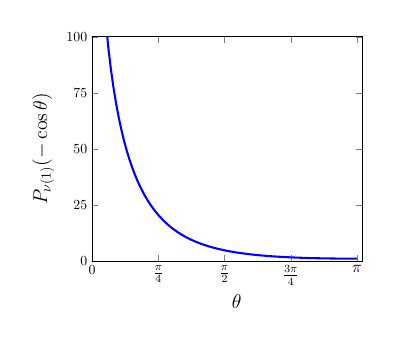
\begin{tikzpicture}[scale=0.5]

\begin{axis}[
  xmin = 0,
  xmax = 3.2,
  xtick = {0,0.7854,1.5708,2.3562,3.1416},
  xticklabels =
  {$0$,\large{$\frac{\pi}{4}$},\large{$\frac{\pi}{2}$},\large{$\frac{3\pi}{4}$},\large{$\pi$}},
  xlabel = $\theta$,
  ymin = 0,
  ymax = 100,
  ytick = {0,25,50,75,100},
  yticklabels = {$0$,$25$,$50$,$75$,$100$},
  ylabel = {$P_{\nu(1)}(-\cos\theta)$},
  xlabel style = {xshift = 7pt},
  ylabel style = {yshift = 2pt},
  label style = {font=\Large},
  ]

% adaptive error
\addplot [mark=none,blue,line width=1.5] table{
3.1733e-02 2.2295e+02
6.3467e-02 1.7258e+02
9.5200e-02 1.4355e+02
1.2693e-01 1.2334e+02
1.5867e-01 1.0800e+02
1.9040e-01 9.5773e+01
2.2213e-01 8.5702e+01
2.5387e-01 7.7221e+01
2.8560e-01 6.9958e+01
3.1733e-01 6.3659e+01
3.4907e-01 5.8140e+01
3.8080e-01 5.3266e+01
4.1253e-01 4.8931e+01
4.4427e-01 4.5055e+01
4.7600e-01 4.1572e+01
5.0773e-01 3.8429e+01
5.3947e-01 3.5583e+01
5.7120e-01 3.2998e+01
6.0293e-01 3.0642e+01
6.3467e-01 2.8491e+01
6.6640e-01 2.6522e+01
6.9813e-01 2.4717e+01
7.2986e-01 2.3057e+01
7.6160e-01 2.1530e+01
7.9333e-01 2.0122e+01
8.2506e-01 1.8822e+01
8.5680e-01 1.7621e+01
8.8853e-01 1.6509e+01
9.2026e-01 1.5479e+01
9.5200e-01 1.4523e+01
9.8373e-01 1.3636e+01
1.0155e+00 1.2811e+01
1.0472e+00 1.2044e+01
1.0789e+00 1.1331e+01
1.1107e+00 1.0665e+01
1.1424e+00 1.0045e+01
1.1741e+00 9.4670e+00
1.2059e+00 8.9271e+00
1.2376e+00 8.4226e+00
1.2693e+00 7.9511e+00
1.3011e+00 7.5102e+00
1.3328e+00 7.0975e+00
1.3645e+00 6.7112e+00
1.3963e+00 6.3494e+00
1.4280e+00 6.0103e+00
1.4597e+00 5.6923e+00
1.4915e+00 5.3942e+00
1.5232e+00 5.1143e+00
1.5549e+00 4.8517e+00
1.5867e+00 4.6051e+00
1.6184e+00 4.3734e+00
1.6501e+00 4.1557e+00
1.6819e+00 3.9511e+00
1.7136e+00 3.7587e+00
1.7453e+00 3.5777e+00
1.7771e+00 3.4075e+00
1.8088e+00 3.2474e+00
1.8405e+00 3.0967e+00
1.8723e+00 2.9548e+00
1.9040e+00 2.8213e+00
1.9357e+00 2.6956e+00
1.9675e+00 2.5772e+00
1.9992e+00 2.4657e+00
2.0309e+00 2.3608e+00
2.0627e+00 2.2619e+00
2.0944e+00 2.1689e+00
2.1261e+00 2.0812e+00
2.1579e+00 1.9988e+00
2.1896e+00 1.9211e+00
2.2213e+00 1.8481e+00
2.2531e+00 1.7794e+00
2.2848e+00 1.7148e+00
2.3165e+00 1.6541e+00
2.3483e+00 1.5971e+00
2.3800e+00 1.5436e+00
2.4117e+00 1.4935e+00
2.4435e+00 1.4464e+00
2.4752e+00 1.4025e+00
2.5069e+00 1.3613e+00
2.5387e+00 1.3230e+00
2.5704e+00 1.2872e+00
2.6021e+00 1.2540e+00
2.6339e+00 1.2231e+00
2.6656e+00 1.1946e+00
2.6973e+00 1.1683e+00
2.7291e+00 1.1442e+00
2.7608e+00 1.1221e+00
2.7925e+00 1.1020e+00
2.8243e+00 1.0839e+00
2.8560e+00 1.0676e+00
2.8877e+00 1.0532e+00
2.9195e+00 1.0406e+00
2.9512e+00 1.0297e+00
2.9829e+00 1.0206e+00
3.0147e+00 1.0131e+00
3.0464e+00 1.0074e+00
3.0781e+00 1.0033e+00
3.1099e+00 1.0008e+00
3.1416e+00 1.0000e+00
};


\end{axis}

\end{tikzpicture}



  \caption{\label{f:legendreP} The LegendreP function
  $P_{\nu(k)}(-\cos\theta)$, for $\theta \in (0,\pi]$ and $k=1$.}
\end{figure}  
We also recall that $P_{\nu}$ is well-defined for all $\nu \in
\mathbb{C}$, whereas $Q_\nu$ is well-defined for $\nu \not=
0,-1,-2,...$. 

On $\S$, from~\eqref{LegendrePequation} we obtain
\begin{align*}  
  \nu(k):=\frac{-1+\sqrt{1-4k^2}}{2}.
\end{align*}
If $0<k^2<\frac{1}{4}$ then $\nu \in (-1,0)$. If $k^2\geq\frac{1}{4}$ then 
\begin{align*}  
  \nu(k):=\frac{-1+i\sqrt{4k^2-1}}{2}.
\end{align*}

We observe that since $k^{2}>0$, $\nu(k) \notin \mathbb{Z}$. Moreover,
if $k>\frac{1}{2}$ then $Im(\nu)\not=0$.  This is the regime in which we
shall work, and in what follows we shall make this assumption on $k$.
This assumption on $k$ is not essential, but is convenient in both our
analysis and numerical methods.  In particular, it allows us to use
conical functions.  Moreover, in the applications we are considering, we
expect $k$ to be large since $k^{2} = \bigO(1/\Delta t)$.

A further substitution allows us to write~\eqref{LegendrePequation} as
a hypergeometric equation, (see, e.g., Section 7.3,~\cite{lebedev}).
This in turn allows us to write the solution of $\mathcal{D}_k(u)=0$ as 
\begin{align*} 
  u(r_0(\theta)) &= P_{\nu(k)}(-\cos(\theta)) = 
    \tensor[_2]{F}{_1}\left(-\nu(k), \nu(k)+  1; 1; 
      \frac{4-r_0^2(\theta)}{4}\right) \\
    &=\tensor[_2]{F}{_1}\left(-\nu(k), \nu(k)+  1; 1;
    \frac{1+\cos(\theta)}{2}\right).
\end{align*} 
Here, $\tensor[_2]{F}{_1}(a,b;c;z)$ is a hypergeometric function. Since
the argument $\frac{1+\cos(\theta)}{2}$ lies between $-1$ and $1$, and
$a+b = 1$, the representation in terms of the hypergeometric function is
also known as the {\it Ferrers' function of the first
kind},~\cite{fatAbramowitz}. 

\begin{figure}
  \centering
  %\begin{tikzpicture} \begin{axis}[view={0}{90}, xlabel=$x$, ylabel=$y$,
%title=View from top] \addplot3[surf] {x}; \end{axis} \end{tikzpicture}


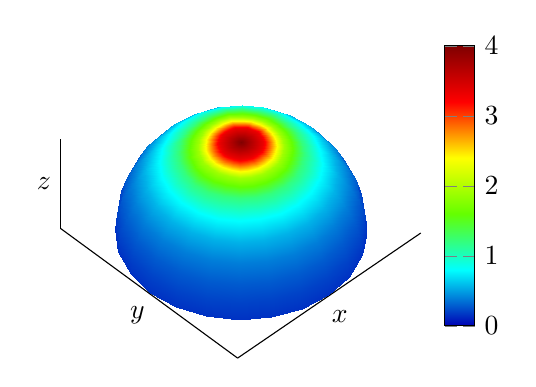
\begin{tikzpicture}

\begin{axis}[%
width=1.8in,
height=2.0in,
view={136}{45},
scale only axis,
axis equal image,
xmin=-1.01,
xmax=1.01,
xtick = \empty,
xlabel = $x$, 
xmajorgrids,
ymin=-1.01,
ymax=1.01,
ytick = \empty,
ylabel = $y$, 
ymajorgrids,
zmin=0,
zmax=1.01,
ztick = \empty,
zlabel = $z$, 
zlabel style={rotate=-90},
zmajorgrids,
axis x line*=bottom,
axis y line*=left,
axis z line*=left,
colormap/bluered,
%colormap={traffic}{color(0cm)=(blue); color(1cm)=(yellow); color(2cm)=(red)},
colorbar,
colorbar style={%title=$\mu$,
        width=0.15in, height=1.4in,
				at={(1.15,0.5)},anchor=east
    },
point meta min=0,
point meta max=4
%point meta min=33651.1920231507,
%point meta max=3000001
]

\addplot3[%
surf,
colormap/bluered,
%colormap={traffic}{color(0cm)=(blue); color(1cm)=(yellow); color(2cm)=(red)},
shader=interp,
draw=black,
point meta=explicit,
mesh/rows=10]
table[row sep=crcr,meta index=3,header=false] {
1.0000e-05 0.0000e+00 1.0000e+00 2.6708e+01\\
9.6593e-06 2.5882e-06 1.0000e+00 2.6708e+01\\
8.6603e-06 5.0000e-06 1.0000e+00 2.6708e+01\\
7.0711e-06 7.0711e-06 1.0000e+00 2.6708e+01\\
5.0000e-06 8.6603e-06 1.0000e+00 2.6708e+01\\
2.5882e-06 9.6593e-06 1.0000e+00 2.6708e+01\\
6.1232e-22 1.0000e-05 1.0000e+00 2.6708e+01\\
-2.5882e-06 9.6593e-06 1.0000e+00 2.6708e+01\\
-5.0000e-06 8.6603e-06 1.0000e+00 2.6708e+01\\
-7.0711e-06 7.0711e-06 1.0000e+00 2.6708e+01\\
-8.6603e-06 5.0000e-06 1.0000e+00 2.6708e+01\\
-9.6593e-06 2.5882e-06 1.0000e+00 2.6708e+01\\
-1.0000e-05 1.2246e-21 1.0000e+00 2.6708e+01\\
-9.6593e-06 -2.5882e-06 1.0000e+00 2.6708e+01\\
-8.6603e-06 -5.0000e-06 1.0000e+00 2.6708e+01\\
-7.0711e-06 -7.0711e-06 1.0000e+00 2.6708e+01\\
-5.0000e-06 -8.6603e-06 1.0000e+00 2.6708e+01\\
-2.5882e-06 -9.6593e-06 1.0000e+00 2.6708e+01\\
-1.8370e-21 -1.0000e-05 1.0000e+00 2.6708e+01\\
2.5882e-06 -9.6593e-06 1.0000e+00 2.6708e+01\\
5.0000e-06 -8.6603e-06 1.0000e+00 2.6708e+01\\
7.0711e-06 -7.0711e-06 1.0000e+00 2.6708e+01\\
8.6603e-06 -5.0000e-06 1.0000e+00 2.6708e+01\\
9.6593e-06 -2.5882e-06 1.0000e+00 2.6708e+01\\
1.0000e-05 -2.4493e-21 1.0000e+00 2.6708e+01\\
1.7365e-01 0.0000e+00 9.8481e-01 3.3287e+00\\
1.6773e-01 4.4943e-02 9.8481e-01 3.3287e+00\\
1.5038e-01 8.6824e-02 9.8481e-01 3.3287e+00\\
1.2279e-01 1.2279e-01 9.8481e-01 3.3287e+00\\
8.6824e-02 1.5038e-01 9.8481e-01 3.3287e+00\\
4.4943e-02 1.6773e-01 9.8481e-01 3.3287e+00\\
1.0633e-17 1.7365e-01 9.8481e-01 3.3287e+00\\
-4.4943e-02 1.6773e-01 9.8481e-01 3.3287e+00\\
-8.6824e-02 1.5038e-01 9.8481e-01 3.3287e+00\\
-1.2279e-01 1.2279e-01 9.8481e-01 3.3287e+00\\
-1.5038e-01 8.6824e-02 9.8481e-01 3.3287e+00\\
-1.6773e-01 4.4943e-02 9.8481e-01 3.3287e+00\\
-1.7365e-01 2.1266e-17 9.8481e-01 3.3287e+00\\
-1.6773e-01 -4.4943e-02 9.8481e-01 3.3287e+00\\
-1.5038e-01 -8.6824e-02 9.8481e-01 3.3287e+00\\
-1.2279e-01 -1.2279e-01 9.8481e-01 3.3287e+00\\
-8.6824e-02 -1.5038e-01 9.8481e-01 3.3287e+00\\
-4.4943e-02 -1.6773e-01 9.8481e-01 3.3287e+00\\
-3.1899e-17 -1.7365e-01 9.8481e-01 3.3287e+00\\
4.4943e-02 -1.6773e-01 9.8481e-01 3.3287e+00\\
8.6824e-02 -1.5038e-01 9.8481e-01 3.3287e+00\\
1.2279e-01 -1.2279e-01 9.8481e-01 3.3287e+00\\
1.5038e-01 -8.6824e-02 9.8481e-01 3.3287e+00\\
1.6773e-01 -4.4943e-02 9.8481e-01 3.3287e+00\\
1.7365e-01 -4.2532e-17 9.8481e-01 3.3287e+00\\
3.4202e-01 0.0000e+00 9.3969e-01 1.9054e+00\\
3.3037e-01 8.8521e-02 9.3969e-01 1.9054e+00\\
2.9620e-01 1.7101e-01 9.3969e-01 1.9054e+00\\
2.4184e-01 2.4184e-01 9.3969e-01 1.9054e+00\\
1.7101e-01 2.9620e-01 9.3969e-01 1.9054e+00\\
8.8521e-02 3.3037e-01 9.3969e-01 1.9054e+00\\
2.0943e-17 3.4202e-01 9.3969e-01 1.9054e+00\\
-8.8521e-02 3.3037e-01 9.3969e-01 1.9054e+00\\
-1.7101e-01 2.9620e-01 9.3969e-01 1.9054e+00\\
-2.4184e-01 2.4184e-01 9.3969e-01 1.9054e+00\\
-2.9620e-01 1.7101e-01 9.3969e-01 1.9054e+00\\
-3.3037e-01 8.8521e-02 9.3969e-01 1.9054e+00\\
-3.4202e-01 4.1885e-17 9.3969e-01 1.9054e+00\\
-3.3037e-01 -8.8521e-02 9.3969e-01 1.9054e+00\\
-2.9620e-01 -1.7101e-01 9.3969e-01 1.9054e+00\\
-2.4184e-01 -2.4184e-01 9.3969e-01 1.9054e+00\\
-1.7101e-01 -2.9620e-01 9.3969e-01 1.9054e+00\\
-8.8521e-02 -3.3037e-01 9.3969e-01 1.9054e+00\\
-6.2828e-17 -3.4202e-01 9.3969e-01 1.9054e+00\\
8.8521e-02 -3.3037e-01 9.3969e-01 1.9054e+00\\
1.7101e-01 -2.9620e-01 9.3969e-01 1.9054e+00\\
2.4184e-01 -2.4184e-01 9.3969e-01 1.9054e+00\\
2.9620e-01 -1.7101e-01 9.3969e-01 1.9054e+00\\
3.3037e-01 -8.8521e-02 9.3969e-01 1.9054e+00\\
3.4202e-01 -8.3771e-17 9.3969e-01 1.9054e+00\\
5.0000e-01 0.0000e+00 8.6603e-01 1.2116e+00\\
4.8296e-01 1.2941e-01 8.6603e-01 1.2116e+00\\
4.3301e-01 2.5000e-01 8.6603e-01 1.2116e+00\\
3.5355e-01 3.5355e-01 8.6603e-01 1.2116e+00\\
2.5000e-01 4.3301e-01 8.6603e-01 1.2116e+00\\
1.2941e-01 4.8296e-01 8.6603e-01 1.2116e+00\\
3.0616e-17 5.0000e-01 8.6603e-01 1.2116e+00\\
-1.2941e-01 4.8296e-01 8.6603e-01 1.2116e+00\\
-2.5000e-01 4.3301e-01 8.6603e-01 1.2116e+00\\
-3.5355e-01 3.5355e-01 8.6603e-01 1.2116e+00\\
-4.3301e-01 2.5000e-01 8.6603e-01 1.2116e+00\\
-4.8296e-01 1.2941e-01 8.6603e-01 1.2116e+00\\
-5.0000e-01 6.1232e-17 8.6603e-01 1.2116e+00\\
-4.8296e-01 -1.2941e-01 8.6603e-01 1.2116e+00\\
-4.3301e-01 -2.5000e-01 8.6603e-01 1.2116e+00\\
-3.5355e-01 -3.5355e-01 8.6603e-01 1.2116e+00\\
-2.5000e-01 -4.3301e-01 8.6603e-01 1.2116e+00\\
-1.2941e-01 -4.8296e-01 8.6603e-01 1.2116e+00\\
-9.1849e-17 -5.0000e-01 8.6603e-01 1.2116e+00\\
1.2941e-01 -4.8296e-01 8.6603e-01 1.2116e+00\\
2.5000e-01 -4.3301e-01 8.6603e-01 1.2116e+00\\
3.5355e-01 -3.5355e-01 8.6603e-01 1.2116e+00\\
4.3301e-01 -2.5000e-01 8.6603e-01 1.2116e+00\\
4.8296e-01 -1.2941e-01 8.6603e-01 1.2116e+00\\
5.0000e-01 -1.2246e-16 8.6603e-01 1.2116e+00\\
6.4279e-01 0.0000e+00 7.6604e-01 8.1002e-01\\
6.2089e-01 1.6637e-01 7.6604e-01 8.1002e-01\\
5.5667e-01 3.2139e-01 7.6604e-01 8.1002e-01\\
4.5452e-01 4.5452e-01 7.6604e-01 8.1002e-01\\
3.2139e-01 5.5667e-01 7.6604e-01 8.1002e-01\\
1.6637e-01 6.2089e-01 7.6604e-01 8.1002e-01\\
3.9359e-17 6.4279e-01 7.6604e-01 8.1002e-01\\
-1.6637e-01 6.2089e-01 7.6604e-01 8.1002e-01\\
-3.2139e-01 5.5667e-01 7.6604e-01 8.1002e-01\\
-4.5452e-01 4.5452e-01 7.6604e-01 8.1002e-01\\
-5.5667e-01 3.2139e-01 7.6604e-01 8.1002e-01\\
-6.2089e-01 1.6637e-01 7.6604e-01 8.1002e-01\\
-6.4279e-01 7.8719e-17 7.6604e-01 8.1002e-01\\
-6.2089e-01 -1.6637e-01 7.6604e-01 8.1002e-01\\
-5.5667e-01 -3.2139e-01 7.6604e-01 8.1002e-01\\
-4.5452e-01 -4.5452e-01 7.6604e-01 8.1002e-01\\
-3.2139e-01 -5.5667e-01 7.6604e-01 8.1002e-01\\
-1.6637e-01 -6.2089e-01 7.6604e-01 8.1002e-01\\
-1.1808e-16 -6.4279e-01 7.6604e-01 8.1002e-01\\
1.6637e-01 -6.2089e-01 7.6604e-01 8.1002e-01\\
3.2139e-01 -5.5667e-01 7.6604e-01 8.1002e-01\\
4.5452e-01 -4.5452e-01 7.6604e-01 8.1002e-01\\
5.5667e-01 -3.2139e-01 7.6604e-01 8.1002e-01\\
6.2089e-01 -1.6637e-01 7.6604e-01 8.1002e-01\\
6.4279e-01 -1.5744e-16 7.6604e-01 8.1002e-01\\
7.6604e-01 0.0000e+00 6.4279e-01 5.5890e-01\\
7.3994e-01 1.9827e-01 6.4279e-01 5.5890e-01\\
6.6341e-01 3.8302e-01 6.4279e-01 5.5890e-01\\
5.4168e-01 5.4168e-01 6.4279e-01 5.5890e-01\\
3.8302e-01 6.6341e-01 6.4279e-01 5.5890e-01\\
1.9827e-01 7.3994e-01 6.4279e-01 5.5890e-01\\
4.6907e-17 7.6604e-01 6.4279e-01 5.5890e-01\\
-1.9827e-01 7.3994e-01 6.4279e-01 5.5890e-01\\
-3.8302e-01 6.6341e-01 6.4279e-01 5.5890e-01\\
-5.4168e-01 5.4168e-01 6.4279e-01 5.5890e-01\\
-6.6341e-01 3.8302e-01 6.4279e-01 5.5890e-01\\
-7.3994e-01 1.9827e-01 6.4279e-01 5.5890e-01\\
-7.6604e-01 9.3813e-17 6.4279e-01 5.5890e-01\\
-7.3994e-01 -1.9827e-01 6.4279e-01 5.5890e-01\\
-6.6341e-01 -3.8302e-01 6.4279e-01 5.5890e-01\\
-5.4168e-01 -5.4168e-01 6.4279e-01 5.5890e-01\\
-3.8302e-01 -6.6341e-01 6.4279e-01 5.5890e-01\\
-1.9827e-01 -7.3994e-01 6.4279e-01 5.5890e-01\\
-1.4072e-16 -7.6604e-01 6.4279e-01 5.5890e-01\\
1.9827e-01 -7.3994e-01 6.4279e-01 5.5890e-01\\
3.8302e-01 -6.6341e-01 6.4279e-01 5.5890e-01\\
5.4168e-01 -5.4168e-01 6.4279e-01 5.5890e-01\\
6.6341e-01 -3.8302e-01 6.4279e-01 5.5890e-01\\
7.3994e-01 -1.9827e-01 6.4279e-01 5.5890e-01\\
7.6604e-01 -1.8763e-16 6.4279e-01 5.5890e-01\\
8.6603e-01 0.0000e+00 5.0000e-01 3.9472e-01\\
8.3652e-01 2.2414e-01 5.0000e-01 3.9472e-01\\
7.5000e-01 4.3301e-01 5.0000e-01 3.9472e-01\\
6.1237e-01 6.1237e-01 5.0000e-01 3.9472e-01\\
4.3301e-01 7.5000e-01 5.0000e-01 3.9472e-01\\
2.2414e-01 8.3652e-01 5.0000e-01 3.9472e-01\\
5.3029e-17 8.6603e-01 5.0000e-01 3.9472e-01\\
-2.2414e-01 8.3652e-01 5.0000e-01 3.9472e-01\\
-4.3301e-01 7.5000e-01 5.0000e-01 3.9472e-01\\
-6.1237e-01 6.1237e-01 5.0000e-01 3.9472e-01\\
-7.5000e-01 4.3301e-01 5.0000e-01 3.9472e-01\\
-8.3652e-01 2.2414e-01 5.0000e-01 3.9472e-01\\
-8.6603e-01 1.0606e-16 5.0000e-01 3.9472e-01\\
-8.3652e-01 -2.2414e-01 5.0000e-01 3.9472e-01\\
-7.5000e-01 -4.3301e-01 5.0000e-01 3.9472e-01\\
-6.1237e-01 -6.1237e-01 5.0000e-01 3.9472e-01\\
-4.3301e-01 -7.5000e-01 5.0000e-01 3.9472e-01\\
-2.2414e-01 -8.3652e-01 5.0000e-01 3.9472e-01\\
-1.5909e-16 -8.6603e-01 5.0000e-01 3.9472e-01\\
2.2414e-01 -8.3652e-01 5.0000e-01 3.9472e-01\\
4.3301e-01 -7.5000e-01 5.0000e-01 3.9472e-01\\
6.1237e-01 -6.1237e-01 5.0000e-01 3.9472e-01\\
7.5000e-01 -4.3301e-01 5.0000e-01 3.9472e-01\\
8.3652e-01 -2.2414e-01 5.0000e-01 3.9472e-01\\
8.6603e-01 -2.1212e-16 5.0000e-01 3.9472e-01\\
9.3969e-01 0.0000e+00 3.4202e-01 2.8415e-01\\
9.0767e-01 2.4321e-01 3.4202e-01 2.8415e-01\\
8.1380e-01 4.6985e-01 3.4202e-01 2.8415e-01\\
6.6446e-01 6.6446e-01 3.4202e-01 2.8415e-01\\
4.6985e-01 8.1380e-01 3.4202e-01 2.8415e-01\\
2.4321e-01 9.0767e-01 3.4202e-01 2.8415e-01\\
5.7540e-17 9.3969e-01 3.4202e-01 2.8415e-01\\
-2.4321e-01 9.0767e-01 3.4202e-01 2.8415e-01\\
-4.6985e-01 8.1380e-01 3.4202e-01 2.8415e-01\\
-6.6446e-01 6.6446e-01 3.4202e-01 2.8415e-01\\
-8.1380e-01 4.6985e-01 3.4202e-01 2.8415e-01\\
-9.0767e-01 2.4321e-01 3.4202e-01 2.8415e-01\\
-9.3969e-01 1.1508e-16 3.4202e-01 2.8415e-01\\
-9.0767e-01 -2.4321e-01 3.4202e-01 2.8415e-01\\
-8.1380e-01 -4.6985e-01 3.4202e-01 2.8415e-01\\
-6.6446e-01 -6.6446e-01 3.4202e-01 2.8415e-01\\
-4.6985e-01 -8.1380e-01 3.4202e-01 2.8415e-01\\
-2.4321e-01 -9.0767e-01 3.4202e-01 2.8415e-01\\
-1.7262e-16 -9.3969e-01 3.4202e-01 2.8415e-01\\
2.4321e-01 -9.0767e-01 3.4202e-01 2.8415e-01\\
4.6985e-01 -8.1380e-01 3.4202e-01 2.8415e-01\\
6.6446e-01 -6.6446e-01 3.4202e-01 2.8415e-01\\
8.1380e-01 -4.6985e-01 3.4202e-01 2.8415e-01\\
9.0767e-01 -2.4321e-01 3.4202e-01 2.8415e-01\\
9.3969e-01 -2.3016e-16 3.4202e-01 2.8415e-01\\
9.8481e-01 0.0000e+00 1.7365e-01 2.0808e-01\\
9.5125e-01 2.5489e-01 1.7365e-01 2.0808e-01\\
8.5287e-01 4.9240e-01 1.7365e-01 2.0808e-01\\
6.9636e-01 6.9636e-01 1.7365e-01 2.0808e-01\\
4.9240e-01 8.5287e-01 1.7365e-01 2.0808e-01\\
2.5489e-01 9.5125e-01 1.7365e-01 2.0808e-01\\
6.0302e-17 9.8481e-01 1.7365e-01 2.0808e-01\\
-2.5489e-01 9.5125e-01 1.7365e-01 2.0808e-01\\
-4.9240e-01 8.5287e-01 1.7365e-01 2.0808e-01\\
-6.9636e-01 6.9636e-01 1.7365e-01 2.0808e-01\\
-8.5287e-01 4.9240e-01 1.7365e-01 2.0808e-01\\
-9.5125e-01 2.5489e-01 1.7365e-01 2.0808e-01\\
-9.8481e-01 1.2060e-16 1.7365e-01 2.0808e-01\\
-9.5125e-01 -2.5489e-01 1.7365e-01 2.0808e-01\\
-8.5287e-01 -4.9240e-01 1.7365e-01 2.0808e-01\\
-6.9636e-01 -6.9636e-01 1.7365e-01 2.0808e-01\\
-4.9240e-01 -8.5287e-01 1.7365e-01 2.0808e-01\\
-2.5489e-01 -9.5125e-01 1.7365e-01 2.0808e-01\\
-1.8091e-16 -9.8481e-01 1.7365e-01 2.0808e-01\\
2.5489e-01 -9.5125e-01 1.7365e-01 2.0808e-01\\
4.9240e-01 -8.5287e-01 1.7365e-01 2.0808e-01\\
6.9636e-01 -6.9636e-01 1.7365e-01 2.0808e-01\\
8.5287e-01 -4.9240e-01 1.7365e-01 2.0808e-01\\
9.5125e-01 -2.5489e-01 1.7365e-01 2.0808e-01\\
9.8481e-01 -2.4121e-16 1.7365e-01 2.0808e-01\\
1.0000e+00 0.0000e+00 6.1232e-17 1.5490e-01\\
9.6593e-01 2.5882e-01 6.1232e-17 1.5490e-01\\
8.6603e-01 5.0000e-01 6.1232e-17 1.5490e-01\\
7.0711e-01 7.0711e-01 6.1232e-17 1.5490e-01\\
5.0000e-01 8.6603e-01 6.1232e-17 1.5490e-01\\
2.5882e-01 9.6593e-01 6.1232e-17 1.5490e-01\\
6.1232e-17 1.0000e+00 6.1232e-17 1.5490e-01\\
-2.5882e-01 9.6593e-01 6.1232e-17 1.5490e-01\\
-5.0000e-01 8.6603e-01 6.1232e-17 1.5490e-01\\
-7.0711e-01 7.0711e-01 6.1232e-17 1.5490e-01\\
-8.6603e-01 5.0000e-01 6.1232e-17 1.5490e-01\\
-9.6593e-01 2.5882e-01 6.1232e-17 1.5490e-01\\
-1.0000e+00 1.2246e-16 6.1232e-17 1.5490e-01\\
-9.6593e-01 -2.5882e-01 6.1232e-17 1.5490e-01\\
-8.6603e-01 -5.0000e-01 6.1232e-17 1.5490e-01\\
-7.0711e-01 -7.0711e-01 6.1232e-17 1.5490e-01\\
-5.0000e-01 -8.6603e-01 6.1232e-17 1.5490e-01\\
-2.5882e-01 -9.6593e-01 6.1232e-17 1.5490e-01\\
-1.8370e-16 -1.0000e+00 6.1232e-17 1.5490e-01\\
2.5882e-01 -9.6593e-01 6.1232e-17 1.5490e-01\\
5.0000e-01 -8.6603e-01 6.1232e-17 1.5490e-01\\
7.0711e-01 -7.0711e-01 6.1232e-17 1.5490e-01\\
8.6603e-01 -5.0000e-01 6.1232e-17 1.5490e-01\\
9.6593e-01 -2.5882e-01 6.1232e-17 1.5490e-01\\
1.0000e+00 -2.4493e-16 6.1232e-17 1.5490e-01\\
};

\end{axis}
\end{tikzpicture}%

  \caption{\label{f:greensFun} $G_1(x,x_0)$ when $x_0=(0,0,1)^T$. The
  singularity at the north pole is logarithmic. Only the top hemisphere
  is shown here for purpose of illustration.}
\end{figure}
A more (computationally) convenient representation is in terms of the
{\it conical or Mehler functions} (Section 8.5 in~\cite{lebedev}). The
conical function $P_{-\frac{1}{2}+ i \tau}(z)$ of order $\tau\in
\mathbb{R}$ solves the equation
\begin{align*}
  (1-z^2)\,w'' -2zw' - \left( \tau^2+\frac{1}{4}\right) \,w = 0.
\end{align*}
In our specific case, we would pick $\tau = \tau(k)$ such that
$\tau^2+\frac{1}{4}=k^2 = -\nu(\nu+1).$  It follows that 
\begin{align*}
  \tau:=\frac{\sqrt{4k^2-1}}{2} \Rightarrow  \nu= -\frac{1}{2}+i\tau, 
\end{align*}
and the solution of $\mathcal{D}_k(u)=0$ is $
  P_{\nu} (-\cos(\theta)) = P_{-\frac{1}{2} + i \tau} 
    (-\cos(\theta)).$
The calculations above lead us then to the following definition:

\begin{definition}
\label{fundamentaldef} 
The fundamental solution for the Yukawa-Beltrami operator $-\lap_\S +
k^2$ for points $x,x_0$ on the surface of the unit sphere is 
\begin{subequations}
  \begin{align}
    G_k(x,x_{0})&:=\C P_{\nu}\left(-<x,x_{0}>\right) \nonumber \\
    &=\C P_{\nu}\left(\frac{\|x-x_{0}\|^2}{2}-1\right) \label{LegP} \\
    &= \C\, \tensor[_2]{F}{_1} \left(-\nu, \nu+1; 1; 
      \frac{1+<x,x_{0}>}{2}\right)\label{hyperG} \\
    &=\C P_{-\frac{1}{2} + i \tau}
    \left(<x,x_{0}>\right) \label{conicalP},
  \end{align} 
\end{subequations}
where 
$\nu:=\frac{-1+i\sqrt{4k^2-1}}{2}$, $k>1/2$, and 
\begin{align}
  \label{constant-definition}    
  \C=-\frac{1}{4\sin(\nu\pi)} 
    =\frac{1}{4\cosh(\frac{\pi}{2}\sqrt{4k^2-1})}.
\end{align}
\end{definition} 
(See Figure~\ref{f:greensFun} for a visualization of $G_1(x,x_0)$.) We
mention here that the specific choice of $\C$ is motivated by the
calculations performed while deriving a representation formula.  We will
see that $\C$ is well-defined with our assumption that $k>1/2$ in
Lemma~\ref{lem:constantC}.


%%%%%%%%%%%%%%%%%%%%%%%%%%%%%%%%%%%%%%%%%%%%%%%%%%%%%%%%%%%%%%%%%%%%%%%%
\subsection{Properties of the fundamental solution of the
Yukawa-Beltrami operator}
Before we embark on the definition and analysis of boundary integral
operators, we examine some properties of the fundamental solution $G_k$
defined in Definition~\ref{fundamentaldef}. We shall use either the
representation~\eqref{LegP},~\eqref{hyperG}, or~\eqref{conicalP} as
convenient.  We first observe that the fundamental solution is symmetric
in its arguments, $G_k(x,x_{0}) = G_k(x_{0},x)$. Next, by noting the
expansion for the conical functions as~\cite{lebedev}
\begin{align*}
  P_{-\frac{1}{2}+i \tau} (\cos(t)) &= 1+
    \frac{4\tau^2+1}{2^2}\sin^2(t/2) + 
      \frac{(4\tau^2+1)(4\tau^2+3^2)}{2^24^2}\sin^4(t/2) + 
    \cdots,
\end{align*}
for $0\leq t\leq \pi$, we see that $G_k(x,x_0)$ does not change sign for
  all $x,x_{0} \in \S, x \neq x_{0}$, provided $k$ is fixed.

Next, we examine the asymptotic behaviour as $x\rightarrow x_0$. In this
case, it is convenient to work with~\eqref{LegP}. Setting $\mu=0$ in
14.8.1 of~\cite{fatAbramowitz} (or using 7.5.5 in~\cite{lebedev}), we
have the asymptotic behaviour
\begin{align} 
  \label{Pasymptotics}
  \lim_{t\rightarrow 1^- } P_\nu(t)&= \frac{1}{\Gamma(1)}=1.
\end{align}
Next, following~\cite{fatAbramowitz}, as $t\rightarrow 1^{-}$,
\begin{align*}
  Q_{\nu}(t)=\frac{1}{2}\log\left(\frac{2}{1-t}\right)-\gamma
  -\psi(\nu+1)+\bigO(1-t),\: \nu \neq -1,-2,...
\end{align*} 
where $\psi(x)$ is the digamma function, $\gamma=0.5772\ldots$ is
Euler's constant, and $Q_{\nu}$ is the other linearly independent
solution of Legendre's equation~\eqref{LegendrePequation}.  For
subsequent use, we denote 
\begin{align*}
  R(\nu):= \frac{1}{2}\log(2) -\gamma -\psi(\nu+1), 
\end{align*}
and therefore for $t$ close to $1$,
\begin{equation}
  \label{Qasymptotics}
  Q_{\nu}(t)=-\frac{1}{2}\log(1-t) + 
  R(\nu) + \bigO(1-t),\: \nu \neq -1,-2,... 
\end{equation}

Now, as $x\rightarrow x_{0}$ on the surface of the sphere,
using~\eqref{LegP} we have 
\begin{align*}
  \lim_{x\rightarrow x_{0}}G_k(x,x_{0}) =
  \C\lim_{x\rightarrow x_{0}} P_{\nu(k)}\left(-<x,x_{0}>\right) =
  \C\lim_{t\rightarrow 1^-}P_{\nu(k)}\left(-t\right).
\end{align*}
We cannot immediately use~\eqref{Pasymptotics}. Instead, we must use the
connection formula 14.9.10 in~\cite{fatAbramowitz} (again setting
$\mu=0$):
\begin{align}
  \frac{2}{\pi}\sin(\nu \pi)Q_\nu(t)= \cos(\nu\pi)P_\nu(t) - P_\nu(-t).
  \label{connect}
\end{align}
Combining~\eqref{connect} with~\eqref{Pasymptotics}
and~\eqref{Qasymptotics}, we obtain
\begin{align}
  \lim_{x\rightarrow x_{0}}G_k(x,x_{0}) &= \lim_{x\rightarrow x_{0}}
      \C P_{\nu}(-<x,x_{0}>) \nonumber \\
  &= \lim_{x\rightarrow x_{0} }\C\left(\cos(\nu\pi)
  P_{\nu}(<x,x_{0}>) - 
      \frac{2}{\pi}\sin(\nu \pi)Q_{\nu}(<x,x_0>)\right) \nonumber \\
  &= \C\cos(\nu\pi) \nonumber \\
  & \quad - \frac{2\C}{\pi}\sin(\nu\pi)\lim_{x\rightarrow x_0} 
      \left(-\frac{1}{2}\log(1-<x,x_0>) + R(\nu) +
      \bigO(1-<x,x_0>)\right) \nonumber \\
  &=\frac{\C\sin(\nu\pi)}{\pi}\lim_{x\rightarrow x_0}
      \log(1-<x,x_0>) + \C\left[\cos(\nu\pi)-
      2\frac{\sin(\nu\pi)}{\pi}R(\nu)\right].
  \label{e:logSingularity}
\end{align}
Therefore, as $x\rightarrow x_{0}$ $G_k(x,x_{0})$ possesses a
logarithmic singularity (recall that $\nu$ is not an integer).  At this
point, we could predict a value for $\C$ so that the strength the
singularity is consistent with that for the
Laplace-Beltrami~\cite{gemmrich}.  However, we compute $\C$ rigorously
below.

It is also useful to document the relation, obtained using recurrence
relations for the LegendreP function (Section 14.10.4
in~\cite{fatAbramowitz}):
\begin{align*} 
  (1-z^2) P'_\nu(z) = (-\nu-1) P_{\nu+1}(z) + (\nu+1)z P_\nu(z).
\end{align*}
Suppose, again without loss of generality, that $x_0$ is the North Pole.
Let $x=x(\theta,\phi)$. Then, $G_k(x,x_0) = \C P_\nu(-\cos(\theta))$,
and
\begin{align}
  \label{difflegp} 
  \frac{d}{d\theta} P_\nu(-\cos(\theta)) =  
    (\nu+1)(\sin\theta) \left( \frac{ P_{\nu+1}(-z) +z
        P_{\nu}(-z)}{z^2-1} 
   \right)\vert_{z=\cos(\theta)}.
\end{align}
Now, using~\eqref{difflegp}, 
\begin{align*}
  \underline{\mbox{curl}}_{\S} G_k(x,x_0)&=-
  \C\frac{\partial}{\partial \theta} \left[P_{\nu(k)}(-\cos(\theta))
  \right] \vec{e}_\varphi \\
  &=-\C(\nu+1)\frac{\sin(\theta)}{\cos^2\theta -1} 
    \left[ P_{\nu+1}(-z) + 
   z 
    P_\nu(-z)\right]\vert_{z=\cos(\theta)} \vec{e}_\varphi. \\
\end{align*}
Since the line element on the surface of the sphere is given by
\begin{align*}
  \vec{t}(x(\varphi,\theta))\cdot ds_{x(\varphi,\theta)} = 
    d\theta\,\vec{e}_{\theta} \,+
    \, \sin\theta d\varphi \,\vec{e}_{\varphi}, 
\end{align*} 
we obtain that
\begin{align}
  \label{curlT}
  \underline{\mbox{curl}}_{\S} G_k(x,x_0)\cdot \vec{t} &= 
  \C (\nu+1)  \left[ P_{\nu+1}(-z) + 
  z P_\nu(-z)\right]\vert_{z=\cos(\theta)} d\phi =: F(\theta)d\phi.
\end{align}
The term $F(\theta)= \C (\nu+1)  \left[ P_{\nu+1}(-z) + z
P_\nu(-z)\right]\vert_{z=\cos(\theta)}$ will be important in subsequent
sections, and is related to the kernel of the second layer operator.
(We shall define this operator carefully later.) For now, however, we
are interested in the limit of $F(\theta)$ as the point $x\rightarrow
x_0$, that is, as $\theta \rightarrow 0^+$.  

\begin{lemma} 
\label{lem:constantC}
Let $F(\theta)$ be as defined in~\eqref{curlT}. Then
$\lim_{\theta\rightarrow 0^+} F(\theta)= \frac{2}{\pi}C_k \sin(\nu
\pi)$.
\end{lemma}
\begin{proof} 
Using~\eqref{connect}, the term in the square bracket of
\begin{align*}
F(\theta) =  \C (\nu+1)  \left[ P_{\nu+1}(-z) + 
  z P_\nu(-z)\right]\vert_{z=\cos(\theta)},
\end{align*}
can be simplified.  Denoting $\cos(\theta)=z$, 
\begin{align}
  P_{\nu+1}(-z) + z P_\nu(-z)&=-\frac{2}{\pi}\sin\left((\nu+1) \pi\right)Q_{\nu+1}(z)+
    \cos((\nu+1)\pi)P_{\nu+1}(z) \nonumber \\
  & \qquad +z\left[-\frac{2}{\pi}\sin(\nu\pi)Q_\nu\left(z\right)+
    \cos(\nu\pi)P_\nu\left(z\right)  \right] \nonumber \\
  &=-\frac{2}{\pi}\left[z\sin(\nu \pi)Q_\nu\left(z\right) + 
    \sin\left((\nu+1) \pi\right)Q_{\nu+1}\left(z\right)\right]
    \nonumber \\
  & \qquad +\left[ \cos((\nu+1)\pi)P_{\nu+1}\left(z\right) + 
    z\cos(\nu\pi)P_\nu\left(z\right) \right] \nonumber \\
  &=-\frac{2}{\pi}\sin(\nu \pi)\left[ 
    zQ_\nu\left(z\right) - Q_{\nu+1}\left(z\right)\right] 
  + \cos(\nu\pi)\left[
    -P_{\nu+1}\left(z\right)+zP_\nu\left(z\right)\right].
  \label{bigmess1}
\end{align}
 
As $x\rightarrow x_{0}$, i.e., as $\theta \rightarrow 0^{+}$, clearly
$z=\cos(\theta)\rightarrow 1^{-}$. Recall that in this limit, $P_\nu(z)
\rightarrow 1.$ Therefore, the terms involving the LegendreP functions
of the first kind in~\eqref{bigmess1} behave as 
\begin{align} 
  \label{smallermess1}
  \lim_{z \rightarrow 1^- }\cos(\nu\pi)\left[ -P_{\nu+1}(z)+ z P_\nu(z)
  \right]  = 0.
\end{align}
We can use~\eqref{Pasymptotics} to compute the limit of the term
involving the Legendre functions of the second kind in~\eqref{bigmess1}:
\begin{align}
  \lim_{z \rightarrow 1^{-}} 
    -\frac{2}{\pi}\sin(\nu\pi)\left[zQ_\nu\left(z\right) - 
    Q_{\nu+1}\left(z\right)\right] 
  &= -\frac{2}{\pi}\sin(\nu\pi)\left[
    \psi(\nu+2)-\psi(\nu+1) \right] \nonumber \\
  &= -\frac{2}{\pi (\nu+1)}\sin(\nu \pi).
  \label{smallermess2}
\end{align}
Putting together~\eqref{smallermess1},~\eqref{smallermess2},
and~\eqref{curlT}, we have
\begin{align} 
  \label{doublelayerwithz}
\lim_{\theta \rightarrow 0^+}F(\theta) 
  = \lim_{z\rightarrow 1-}\C(\nu+1)\left[ P_{\nu+1}(-z)+zP{\nu}(-z)\right]
  = \C \frac{2}{\pi} \sin(\nu \pi).
\end{align}
\end{proof}
\qed

Observe that setting $\C=-\frac{1}{4\sin(\nu \pi)}$, that is, using
exactly the constant defined in~\eqref{constant-definition} in the
definition of $G_k(x,x_0)$, we have $\lim_{\theta\rightarrow
0^+}F(\theta)=\frac{1}{2\pi}.$  While this formulation is a
normalization of the second layer potential (defined in the next
section), it is equivalent to imposing that $G(x,x_{0})$ is the
fundamental solution of the Yukawa-Beltrami equation.  That is, this
choice of $C_{k}$ guarantees that $(-\Delta_{\S} + k^{2})G_{k}(x,x_{0})
= \delta(x-x_{0})$, where $\delta$ is the usual Dirac distribution.

The following representation formula can be found in~\cite{mit:tay1999}
(equation (7.37)).  Let $\Omega$ and
$\Omega^{c}:=\S\setminus{\overline{\Omega}}$ be a simply-connected
submanifold and its complement on the sphere. 
\begin{proposition}
\label{prop:repr}
Every sufficiently smooth function $u \in C^{2}(\Omega) \cap
C^{1}(\overline{\Omega})$ satisfies the representation formula
\begin{align} 
\label{eq:representationformula}
 - \int\limits_{\Omega} 
    G_k(x,x_{0})\left[\lap_{\S}u(x) -k^2 u(x)\right]\,d\sigma_x 
 &- \int\limits_{{\Gamma}} G_k(x,x_{0})  
    \underline{\mbox{curl}}_{\S} u(x) \cdot \vec{t}(x) ds_x \nonumber \\
 + \int\limits_{{\Gamma}}  u(x)
 \,\underline{\mbox{curl}}_{{\S}} G_k(x,x_0) \cdot \vec{t}(x) ds_x 
 &= \left\{ \begin{array}{ll} u(x_0) & \mbox{ if $x_0\in \Omega$},\\
  0 & \mbox{ if  $x_0\in{\Omega}_c$}. 
  \end{array} \right.
\end{align}
\end{proposition}


%%%%%%%%%%%%%%%%%%%%%%%%%%%%%%%%%%%%%%%%%%%%%%%%%%%%%%%%%%%%%%%%%%%%%%%%
\section{Layer potentials and boundary integral operators}
Now that we have the fundamental solution $G_k(x,x_0)$ defined in
Definition~\ref{fundamentaldef} for the Yukawa-Beltrami equation and a
representation formula~\eqref{eq:representationformula}, we can define
convenient layer potentials which in turn will be used to reduce the
boundary value problem~\eqref{DBVP} over the domain $\Omega$ to a
boundary integral equation over $\Gamma = \partial \Omega$.


%%%%%%%%%%%%%%%%%%%%%%%%%%%%%%%%%%%%%%%%%%%%%%%%%%%%%%%%%%%%%%%%%%%%%%%%
\subsection{Single- and double-layer potentials}
We define the following two layer potentials:
\begin{itemize}
\item the {\bf single-layer potential} with sufficiently smooth density
function $\sigma$
  \begin{align}
    (\widetilde{V_k}\sigma)(x):=\int\limits_{\Gamma}
    G_k(x,y)\,\sigma(y)\,ds_y,\quad\mbox{for $x \notin \Gamma$};
    \label{singlelayerpotential}
  \end{align}
\item and the {\bf double-layer potential} with sufficiently smooth
density function $\mu$
  \begin{align}
    (\widetilde{W_k}\mu )(x):=\int\limits_{\Gamma}
    \mu(y)\,[\underline{\mbox{curl}}_{\S} G_k(x,y)\cdot \vec{t}(y)]\,
    ds_y, \quad\mbox{for $x\notin\Gamma$}.
    \label{doublelayerpotential}
  \end{align}
\end{itemize}
We wish to point out here that the form of the double-layer potential
above is equivalent to the, perhaps, more familiar form:
\begin{align*}
  (\widetilde{W_k}\mu )(x):=-\int\limits_{\Gamma}
  \mu(y) \frac{\partial \,}{\partial \mathbf{n}(y)} G_k(x,y) \,
  ds_y, \quad\mbox{for $x\notin\Gamma$},
\end{align*}
where $\mathbf{n}(y)$ is the outward pointing normal to $\Gamma$ at the
point $y$ lying in a tangent plane to $\S$.  See~\cite{kro:nig2013} for
a more detailed discussion on this point.

By Proposition~\ref{prop:repr}, every solution to the homogeneous
Yukawa-Beltrami equation can be written as the sum of a single- and a
double-layer potential.  This  is the starting point for the so-called
direct boundary integral approach. However, for the purpose of this
paper we follow the layer ansatz based on the following observation.

For $x \in \Omega, x \notin \Gamma$, the single-layer
potential~\eqref{singlelayerpotential} satisfies $(-\lap_{\S} + k^{2})
(\widetilde{V_k}\sigma)(x)=0$.  Hence, we may find the general solution
of the Dirichlet boundary value problem~\eqref{DBVP} in terms of a
single-layer potential.  Similarly, the double-layer
potential~\eqref{doublelayerpotential} satisfies $(-\lap_{\S} +
k^2)(\widetilde{W}\mu)(x)=0$.  We might thus also try to look for the
solution to~\eqref{DBVP} in the form of a double-layer potential.  In
either case, we need to calculate the unknown density.  In order to
formulate a boundary integral equation that $\sigma$ or $\mu$ solves,
we require the jump relations of the layer potentials.


%%%%%%%%%%%%%%%%%%%%%%%%%%%%%%%%%%%%%%%%%%%%%%%%%%%%%%%%%%%%%%%%%%%%%%%%
\subsection{Jump relations for the layer potentials} 
In the previous section, we have only defined the layer potentials for
$x$ away from the boundary curve. However, in order to align the
operators with the given Dirichlet data along $\Gamma$, we need to
investigate their behavior in the limit as $x$ approaches $\Gamma$.
Similarly, if one is interested in solving the Neumann problem in which
the tangential component of the vectorial surface rotation is prescribed
along $\Gamma$, one has to investigate the limit features of this
quantity for the layer potentials. In both cases, there will be certain
jump relations across the curve $\Gamma$. For the purpose of this paper
however, we will restrict ourselves to the Dirichlet case.  First,
consider the single-layer potential with density $\sigma$ for $x \notin
\Gamma$:
\begin{align*}
  (\widetilde{V_k}\sigma)(x) & =  \int\limits_\Gamma
  G_k(x,y)\,\sigma(y)\,ds_{y} \\
  & = \C \int\limits_\Gamma P_{\nu(k)}(-<x,y>)\,\sigma(y)\,ds_{y}.
\end{align*}
The following Lemma, which is proved in~\cite{mit:tay1999} (Proposition
3.8), describes the limiting behavior of the single-layer potential.
\begin{lemma}
Let $\widetilde{V_k}$ be the single-layer potential defined
in~\eqref{singlelayerpotential}. For $x_{0}\in\Gamma$ we have:
\begin{align*} 
  (V\sigma)(x_0) & := \lim\limits_{\substack{
      x \to x_{0} \\ x \in \Omega}}
  \,(\widetilde{V_k}\sigma)(x) = \int\limits_\Gamma G_k(x_{0},y)\,\sigma(y)\,ds_{y}
\end{align*}
as a weakly singular line integral and hence $(\widetilde{V_k}\sigma)$
is continuous across $\Gamma$.
\end{lemma}

Unlike the single-layer potential, the double-layer potential is
discontinuous across the boundary of the domain.  In particular, we have
the following Lemma which is proved in~\cite{mit:tay1999} (Proposition
3.8).
\begin{lemma} 
\label{l:DLPjump} 
Let $\widetilde{W_k}$ be the double-layer potential defined
in~\eqref{doublelayerpotential}, and let $\gamma_0^{\Omega}$ (resp.
$\gamma_0^{\Omega^c})$ denote the trace operator on $\Gamma$, with
traces from inside (respectively outside) $\Omega$.  For $x_{0} \in
\Gamma$ we have:
\begin{align*} 
  (\gamma^{\Omega^{c}}_0\widetilde{W_k}\mu)(x_0)=
  \lim\limits_{\substack{x \to x_0 \\ x \in \Omega^{c}}}\, 
  (\widetilde{W_k}\mu)(x) =
  (K\mu)(x_0)\,+\,\left(1-\frac{\alpha(x_0)}{2\pi}\right)\,\mu(x_0),
\end{align*}
where $\alpha(x_{0})$ represents the interior (with respect to
$\Omega^{c}$) angle of $\Gamma$ at $x_{0}$. For a smooth curve, $\alpha
= \pi$. The {\it double-layer operator} $K$ is defined via the Cauchy
principle value: 
\begin{align*}
  (K\mu)(x_0)&=\lim_{\varepsilon\rightarrow 0}
  \, (K_{\varepsilon}\mu)(x_0) \quad \mbox{where}\qquad
  (K_{\varepsilon}\mu)(x_0)&:=\int\limits_{y\in C_{\epsilon,\geq}} 
  \mu(y)\,\left[\underline{\mbox{curl}}_{\S}
  \,G_k(x_{0},y)\cdot\vec{t}(y)\right]\,ds_{y}.
\end{align*}
Hence the double-layer potential satisfies:
\begin{align*}
  \left[(\gamma_0\widetilde W_k\mu) \right]_\Gamma := 
  (\gamma^{\Omega^{c}}_0\widetilde W_k\mu)+(\gamma^{\Omega}_{0} 
  \widetilde{W_k}\mu)=\mu,
\end{align*}
where we tacitly assumed the orientation of the tangential vector
$\vec{t}$ along $\Gamma$ to be in accordance with the orientation of
$\Omega^{c}$ in the sense of Stokes' theorem.

\end{lemma}

We need to record one further property of this kernel, which will be
used to understand the convergence properties of our quadrature rule in
Section~\ref{s:numerics}.

\begin{lemma}
\label{regularity}
Let $x_0,x$ be points on the sphere, connected by the smooth curve
$\Gamma$. Let $x_0$ be fixed, and let $\Gamma$ be parametrized by
$x=x(s), s\in[-A,A]$ such that $x(\tau)=x_{0}$. Then the kernel of the
double-layer operator is continuously differentiable in $s$, but the
second derivative is unbounded. More precisely, the function 
\begin{align*}
  f(s,\tau):=\underline{\mbox{curl}}_{\S}\,
    G_{k}(x(\tau),x(s))\cdot\vec{t}(s), \quad s\in[-A,A],
\end{align*}
has the following properties:
\begin{itemize}
\item 
\begin{align*}
  f(s,\tau) = L_{1}(s,\tau) \log(L_{3}(s,t)) + L_{2}(s,\tau),
\end{align*}
where $L_{1}, L_{2}$ and $L_{3}$ are analytic.
\item 
\begin{align*} 
  \lim_{\substack {s \rightarrow \tau}} f(s,\tau) =
    L_{2}(\tau,\tau) =  -\frac{1}{4\pi} 
    \kappa \mathbf{t}\cdot(\mathbf{n}_{0} \times \mathbf{x}_{0}).
\end{align*}

Here $\kappa$ is the principle curvature of $\Gamma$ at $x_{0}$,
$\mathbf{x}_{0}$ is the 3-dimensional vector associated with the point
$x_{0}$ (assuming the origin is located at the center of the sphere),
$\mathbf{n}_{0}$ is the principle normal of $\Gamma$ at $x_0$ and
$\mathbf{t}$ is the tangent vector.
\end{itemize}
\end{lemma}

\begin{proof}
We provide a simple argument via l'H\^{o}pital's rule in the case that
$\Gamma$ is a simple smooth closed curve. For this argument, it is
easier  to work with points and vectors in $\mathbb{R}^3$.  Let $x_{0}$,
$x$ be points on the unit sphere. We identify them with the
3-dimensional vectors $\mathbf{x}_{0}$, $\mathbf{x}$ respectively.  Let
$\mathbf{t}$ and $\mathbf{n}$ be the unit tangent and normal vectors at
the point $\mathbf{x} \in \Gamma$ lying in the tangent plane of
$\mathcal{S}$.  We note for future reference that
$\mathbf{x}=\mathbf{e}_{r}$, $\mathbf{x} \cdot \mathbf{x} = 1$, and
$\mathbf{x}=\mathbf{n} \times \mathbf{t}$. Since $\Gamma$ is
parametrized by arclength $s$, we also note the following identities:

\begin{align*}
  \mathbf{t} = \frac{d\mathbf{x}}{ds}, \qquad 
  \frac{d\mathbf{t}}{ds} = \kappa \, \mathbf{n}.
\end{align*}
The second identity is one of the Frenet formulae, where $\kappa$ is the
curvature of the curve $\Gamma$ at the point $\mathbf{x}$ and
$\mathbf{n}$ is the principal normal to the curve.  From these, it is
straightforward to show that 
\begin{align*}
  \frac{d \, }{ds} \left( \mathbf{t} \times \mathbf{x} \right)=
  \kappa \mathbf{n} \times \mathbf{x} . 
\end{align*}

We now examine the kernel of the double-layer potential. Calculating the
three dimensional gradient of the fundamental solution $G$ yields
\begin{align*}
  \nabla G_k(x(\tau),x(s)) &= \C \nabla P_\nu\left(
    \frac{\|x(\tau)-x(s)\|^2}{2}-1\right) \\
  &=-\C P'_\nu\left(\frac{\|x(\tau)-x(s)\|^2}{2}-1\right)
    (\mathbf{x}(\tau)-\mathbf{x}(s)),
\end{align*}
which we can decompose into the surface gradient plus a derivative in
the radial direction. We can write this more concisely as
\begin{align*}
  \nabla G_{k}(x(\tau),x(s))=-\C P'_{\nu}(z) (\mathbf{x}(\tau)-\mathbf{x}(s)), 
  \qquad \mbox{where}\qquad z=\frac{\|{ x}(\tau)-{x}(s)\|^2}{2}-1.
\end{align*} 

The kernel of the double-layer operator is $f(s,\tau)=
\frac{\partial}{\partial \mathbf{n}} G_{k}({x}_{0},{x})$, which in turn
can be written as 
\begin{align*}
  f(s,\tau)=\frac{\partial \, }{\partial \mathbf{n}} G_{k}(x_{0},x) 
  =\nabla G_{k} \cdot \mathbf{n}
  =-\C P'_{\nu}(z)\left(
    (\mathbf{x}_{0}-\mathbf{x})\cdot \mathbf{n}(s) \right).
\end{align*}
Recalling from~\eqref{difflegp} that
$P'_{\nu}(z)=-\frac{(\nu+1)}{1-z^{2}}(P_{\nu+1}(z)-z P_{\nu}(z))$,
\begin{align}
  f(s,\tau)= \frac{\C(\nu+1)}{1-z^2} \left(
    P_{\nu+1}(z)-zP_{\nu}(z)\right)\left(
  (\mathbf{x}_0-\mathbf{x})\cdot \mathbf{n}(s) \right).
  \label{colton2}
\end{align}
Now, as $s \rightarrow \tau$, $z \rightarrow -1.$ Using the connection
formulae~\eqref{connect}, and denoting $-z = \zeta$, we
rewrite~\eqref{colton2} as
\begin{align}
 f(s,\tau)= \frac{\C(\nu+1)}{1-z^2}&\left(
   (\mathbf{x}_0-\mathbf{x})\cdot \mathbf{n}(s) \right) \nonumber \\
    &\left\{ \frac{2}{\pi}\sin(\nu\pi)
    \left( -\zeta Q_{\nu}(\zeta) + Q_{\nu+1}(\zeta)\right) 
    +\cos(\nu\pi)\left(
    -P_{\nu+1}(\zeta)+\zeta P_\nu(\zeta)\right)\right\}.
\end{align}

We know each term involving the LegendreP function is smooth at
$\zeta=1$.  This can be seen by converting the expressions to
hypergeometric functions with the argument $\frac{1+z}{2}$, which is
analytic as long as $|z+1| < 2$~\cite{fatAbramowitz} (equation 15.2.1).
The terms involving $Q_{\nu}(\zeta)$ are not smooth.
By~\eqref{Qasymptotics}, as $\zeta \rightarrow 1$, we know that $\zeta
Q_\nu(\zeta) - Q_{\nu+1}(\zeta)$ has a singularity of form
$\frac{1-\zeta}{2}\log(1-\zeta)$.  Using this fact, we can write
\begin{align*}
 f(s,\tau)&= L_{1}(s,\tau)\log(L_3(s,\tau)) + L_2(s,\tau), \\
 L_1(s,\tau) &= - \frac{(1+\nu)}{1-\zeta^2}\left(
    (\mathbf{x}_{0}-\mathbf{x})\cdot \mathbf{n}(s) \right) 
    \frac{1}{4\pi}(1-\zeta), \\ 
 L_{3}(s,\tau)&= 1-\zeta = 1+ z = \frac{\|x(\tau) - x(s)\|^2}{2}, \\
 L_{2}(s,\tau)&= f(s,\tau) - L_{1}(s,\tau)\log(L_{3}(s,\tau)).
\end{align*}
It is clear that $L_{1}(s,\tau)$ and $L_{3}(s,\tau)$ are smooth.
Indeed, when $s$ is close to $\tau$, the normal $\mathbf{n}(s)$ becomes
nearly orthogonal to the curve $x(\tau)-x(s)$. Therefore, $f(\tau,\tau)
= L_{2}(\tau,\tau).$  Moreover, by inspection of the series involved in
the definitions of $Q_{\nu},P_{\nu}$, we see that $L_{2}(s,\tau)$ is
also smooth, since we have precisely subtracted the logarithmic
singularity. Note that this argument is very similar to that used
in~\cite{coltonkress}

It remains to precisely compute $f(\tau,\tau)$. To this end, we recall
that from~\eqref{doublelayerwithz},
\begin{align*}
  \C(\nu+1)\lim_{z\rightarrow 1^-} 
    (P_{\nu+1}(-z)+zP_{\nu}(-z)) = -\frac{1}{2\pi}.
\end{align*}
From~\eqref{colton2}, 
\begin{align*}
  \lim_{s\rightarrow \tau}f(s,\tau) = -\frac{1}{2\pi} \lim_{s\rightarrow \tau}
  \frac{(\mathbf{x}_{0}-\mathbf{x})}{\|\mathbf{x}_{0}-\mathbf{x}\|^2} \cdot
  \left(\mathbf{t} \times \mathbf{x} \right) =
  -\frac{1}{2\pi}\lim_{s\rightarrow \tau}q(x(\tau),x(s))
\end{align*}
where
$q(x(\tau),x(s)):=\frac{\mathbf{x}(s)-\mathbf{x}(\tau)}{\|\mathbf{x}(s)-\mathbf{x}(\tau)\|^2}
\cdot \left(\mathbf{t} \times \mathbf{x} \right).$ 

This term can be shown to be continuous as $\mathbf{x} \rightarrow
\mathbf{x}_{0}$ by l'H\^{o}pital's rule.  A first application of
l'H\^{o}pital's rule to evaluate $q(x_{0},x)$ at the point of
singularity, $x = x_{0}$, 
\begin{align*}
  \lim_{x \rightarrow x_{0}}q(x_{0},x) & = 
  \lim_{x \rightarrow x_{0}} 
  \frac{ -\mathbf{t} \cdot \left(\mathbf{t} \times \mathbf{x} \right)
  + (\mathbf{x}_{0}-\mathbf{x}) \cdot \left( \kappa \mathbf{n}
  \times \mathbf{x} \right)}
  {-2(\mathbf{x}_{0} - \mathbf{x}) \cdot \mathbf{t}} \\
  & = \lim_{\mathbf{x} \rightarrow \mathbf{x}_{0}} 
  \frac{(\mathbf{x}_{0}-\mathbf{x}) \cdot \left(
  \kappa\mathbf{n} \times \mathbf{x}\right)}
  {-2(\mathbf{x}_{0} - \mathbf{x}) \cdot \mathbf{t}}. 
\end{align*}
Proceeding with a second application of l'H\^{o}pital's rule yields
\begin{align*}
  \lim_{x \rightarrow x_{0}} q(x_{0},x)  
  & = \lim_{x \rightarrow x_{0}} \frac{-\mathbf{t} \cdot 
  \left( \kappa \mathbf{n} \times \mathbf{x} \right) +
  \mathcal{O}(\mathbf{x} - \mathbf{x}_{0})}
  {-2\mathbf{t} \cdot \mathbf{t} + \mathcal{O}(\mathbf{x}-\mathbf{x}_{0})}
  = \frac{1}{2} \mathbf{t} \cdot \left( \kappa \mathbf{n}_{0} \times 
  \mathbf{x}_{0} \right).
\end{align*}

\end{proof}
\qed

From Lemma~\ref{regularity}, we see that the kernel of the double-layer
operator, $\underline{\mbox{curl}}_{\S}\, G_{k}(x,y)\cdot\vec{t}(y)$,
is continuous at $x \in \Gamma$ as a function of $y$.  This allows us
to conclude that the integral operator $\widetilde{W_k}$ is a compact
operator from $L^{2}(\Gamma)$ to itself.  The compactness, in addition
to the jump $1-\alpha(x_0)/(2\pi)$ (Lemma~\ref{l:DLPjump}) guarantees
that the double-layer potential representation will result in a second
kind Fredholm integral equation with a compact operator.

%%%%%%%%%%%%%%%%%%%%%%%%%%%%%%%%%%%%%%%%%%%%%%%%%%%%%%%%%%%%%%%%%%%%%%%%
\section{Numerical Examples}
\label{s:numerics}
In this section, we apply standard numerical methods to solve the
Fredholm integral equation of the second kind
\begin{align}
  \label{e:dlpBIE}
  \frac{1}{2}\mu(x_{0}) + \int_{\Gamma}
    [\underline{\mbox{curl}}_{\S}G_{k}(x_{0},y) \cdot
    \vec{t}(y)] \mu(y)ds_{y} = g(x_{0}), \quad x_{0} \in \Gamma,
\end{align}
and to evaluate the double-layer potential
\begin{align}
  \label{e:dlpuEval}
  u(x) = \int_{\Gamma} [\underline{\mbox{curl}}_{\S}G_{k}(x,y) 
    \cdot \vec{t}(y)] \mu(y)ds_{y}, \quad x \in \Omega,
\end{align}
where
\begin{align*}
  G_{k}(x,y) = \C P_{\nu(k)} \left(
    \frac{\|x - y\|^{2}}{2} - 1\right), \quad 
  \C=-\frac{1}{4\sin(\nu\pi)}.
\end{align*}
We assume that the boundary $\Gamma$ of the geometry is a smooth
function so that $\alpha(x_{0}) = \pi$, where $\alpha$ is defined in
Lemma~\ref{l:DLPjump}.

In~\eqref{e:dlpuEval}, since $x \notin \Gamma$, the integrand is
periodic and smooth.  Therefore, for a fixed $x\in \Omega$, the
trapezoid rule has spectral accuracy.  However, since the error grows as
$x$ approaches $\Gamma$, our reported errors are only measured at points
$x$ sufficiently far from $\Gamma$.  We test two quadrature formulas for
solving~\eqref{e:dlpBIE}.  First, we test the trapezoid rule which we
expect will achieve third-order accuracy since the integrand is once
continuously differentiable (Lemma~\ref{regularity}).  Second, since we
know that the kernel contains a logarithmic
term~(Lemma~\ref{regularity}), we test a high-order hybrid
Gauss-trapezoidal quadrature formula designed for functions that contain
logarithmic singularities~\cite{alpert}.

For all the examples, we discretize each connected component of the
boundary with $N$ unknowns and solve the resulting linear system with
unrestarted GMRES and a tolerance of $10^{-11}$.  The error of the
Alpert quadrature formula is $\mathcal{O}(h^{16}\log h)$, and we use
Fourier interpolation to assign values to the density function $\mu$ at
quadrature nodes that are intermediate to the regular grid.

We present four numerical examples which we now summarize.
\begin{itemize}
  \item{\em{The effect of the quadrature rule}:} For a two-ply connected
  domain, we report a convergence study for the two quadrature formulas.
  We also establish that the number of GMRES iterations is independent
  of the mesh size.

  \item{\em{The effect of $k$}:} For the same two-ply connected
  domain, we examine the effect of the parameter $k$ on the condition
  number of the linear system corresponding to~\eqref{e:dlpBIE}, and
  its effect on the number of GMRES iterations.

  \item{\em{The effect of the geometry's curvature}:} We consider a
  simply-connected domain and vary the aspect ratio of the major to
  minor axis of the domain's boundary.  We examine the effect of this
  parameter on the conditioning and the number of GMRES iterations.

  \item{\em{A complex domain}:} We demonstrate that our method is able
  to solve the Yukawa-Beltrami equation in complex domains by
  solving~\eqref{DBVP} in a 36-ply connected domain, with an acceptable
  number of GMRES iterations.
\end{itemize}


%%%%%%%%%%%%%%%%%%%%%%%%%%%%%%%%%%%%%%%%%%%%%%%%%%%%%%%%%%%%%%%%%%%%%%%%%
\subsection{The effect of the quadrature rule}
We consider the two-ply connect geometry illustrated in
Figure~\ref{f:twoply}.  An exact solution is formed by taking the
Dirichlet boundary condition corresponding to the sum of two fundamental
solutions centered inside the two islands.  In Table~\ref{t:example1},
we report the number of GMRES iterations (this was independent of the
quadrature formula).  We see that the number of GMRES iterations is
independent of the mesh size, the error of the trapezoid rule has
third-order accuracy, and the error of the Alpert quadrature formula
quickly decays to the GMRES tolerance.

\begin{figure}[htps]
  \includegraphics[width=0.5\textwidth]{Fig1}
  \includegraphics[width=0.5\textwidth]{Fig2}
\caption{\label{f:twoply} A numerical solution of the Yukawa-Beltrami
equation with $k=4$ in a two-ply connected domain viewed from two
different angles.  The exact solution is the sum of two fundamental
solutions, each one centered inside the regions bounded by $\Gamma$.}
\end{figure}

\begin{table}[htps]
\caption{\label{t:example1} The number of GMRES iterations and the
error at a collection of points sufficiently far from $\Gamma$.}
\centering
\begin{tabular*}{0.8\textwidth}{@{\extracolsep{\fill}}lllll}
$N$ & \# GMRES & Trapezoid Error & Alpert Error  \\
\hline\noalign{\smallskip}
32   & 9 & 6.67E-5 & 5.54E-6  \\
64   & 9 & 7.84E-6 & 9.66E-10 \\
128  & 9 & 9.86E-7 & 2.28E-11 \\
256  & 9 & 1.24E-7 & 3.68E-11 \\
512  & 9 & 1.59E-8 & 1.76E-10 \\  
1024 & 9 & 1.84E-9 & 1.20E-10 \\ 
\noalign{\smallskip}\hline
\end{tabular*}
\end{table}

%%%%%%%%%%%%%%%%%%%%%%%%%%%%%%%%%%%%%%%%%%%%%%%%%%%%%%%%%%%%%%%%%%%%%%%%
\subsection{The effect of $k$}
We consider the same two-ply connected geometry illustrated in
Figure~\ref{f:twoply}.  We solve~\eqref{e:dlpBIE} for varying values of
$k > 1/2$ using Alpert's quadrature rule with $N=32$.  We report the
condition number of the resulting linear system and the required number
of GMRES iterations in Table~\ref{t:example2}.  We see that for larger
values of $k$, the conditioning of the linear system improves, and the
number of GMRES iterations decreases.  In Figure~\ref{f:evalues}, we
plot the eigenvalues of the linear system for $k=1$ and $k=64$.  We see
that for larger values of $k$, the eigenvalues cluster more strongly
around $1/2$ resulting in a smaller number of GMRES iterations and a
smaller condition number.

\begin{table}[htps]
\caption{\label{t:example2} The condition number of the linear system
corresponding to a discretization of~\eqref{e:dlpBIE} and the number of
GMRES iterations as a function of the parameter $k$.}
\centering
\begin{tabular*}{0.8\textwidth}{@{\extracolsep{\fill}}lll}
$k$ & Condition Number & \# GMRES \\
\hline\noalign{\smallskip}
0.51 & 4.22E1 & 14 \\
1    & 1.22E1 & 13 \\
2    & 4.50E0 & 11 \\
4    & 2.17E0 & 9  \\
8    & 1.45E0 & 8  \\  
16   & 1.24E0 & 7  \\ 
32   & 1.13E0 & 6  \\
64   & 1.07E0 & 6  \\
\noalign{\smallskip}\hline
\end{tabular*}
\end{table}

\begin{figure}[htps]
\centering
\begin{tabular}{cc}
\begin{tikzpicture}[scale = 0.5]

\begin{axis}[
%  title = {\Large{$k=1$}},
  xmin = 0.0,
  xmax = 0.75,
  xlabel = Real,
  ymin = -3.2e-4,
  ymax = 3.2e-4,
  ylabel = Imag,
  xtick = {0,0.25,0.5,0.75},
  xticklabels = {0,0.25,0.50,0.75},
  ytick = {-3e-4,0,3e-4},
  yticklabels = {-3E-4,0,3E-4},
  scaled x ticks = false,
  scaled y ticks = false
]


\addplot[mark=*,only marks,blue,mark size = 1pt] table{
5.6717e-02 0.0000e+00
1.7831e-01 0.0000e+00
2.8736e-01 0.0000e+00
3.1287e-01 0.0000e+00
6.5195e-01 0.0000e+00
6.4921e-01 0.0000e+00
4.1494e-01 0.0000e+00
5.7632e-01 0.0000e+00
4.3928e-01 0.0000e+00
5.5556e-01 0.0000e+00
4.6404e-01 0.0000e+00
5.3229e-01 0.0000e+00
4.7869e-01 0.0000e+00
5.1984e-01 0.0000e+00
4.8468e-01 0.0000e+00
5.1368e-01 0.0000e+00
4.9254e-01 0.0000e+00
4.9352e-01 0.0000e+00
5.0684e-01 0.0000e+00
5.0563e-01 0.0000e+00
4.9733e-01 0.0000e+00
4.9736e-01 0.0000e+00
5.0218e-01 0.0000e+00
5.0234e-01 0.0000e+00
4.9900e-01 0.0000e+00
5.0073e-01 0.0000e+00
4.9928e-01 0.0000e+00
5.0053e-01 0.0000e+00
4.9958e-01 0.0000e+00
4.9962e-01 0.0000e+00
4.9995e-01 2.8255e-04
4.9995e-01 -2.8255e-04
5.0023e-01 0.0000e+00
4.9980e-01 1.2243e-04
4.9980e-01 -1.2243e-04
4.9979e-01 0.0000e+00
5.0014e-01 1.4779e-04
5.0014e-01 -1.4779e-04
5.0016e-01 0.0000e+00
5.0009e-01 0.0000e+00
4.9990e-01 0.0000e+00
4.9999e-01 8.6180e-05
4.9999e-01 -8.6180e-05
4.9994e-01 0.0000e+00
4.9995e-01 0.0000e+00
4.9996e-01 0.0000e+00
4.9997e-01 0.0000e+00
5.0001e-01 0.0000e+00
5.0001e-01 0.0000e+00
4.9998e-01 0.0000e+00
4.9998e-01 0.0000e+00
4.9998e-01 0.0000e+00
5.0000e-01 5.6716e-07
5.0000e-01 -5.6716e-07
4.9999e-01 4.6911e-06
4.9999e-01 -4.6911e-06
5.0000e-01 0.0000e+00
4.9999e-01 3.1248e-06
4.9999e-01 -3.1248e-06
4.9999e-01 1.4834e-06
4.9999e-01 -1.4834e-06
4.9999e-01 0.0000e+00
4.9999e-01 0.0000e+00
4.9999e-01 0.0000e+00
};
\end{axis}



\end{tikzpicture}
 &
\begin{tikzpicture}[scale = 0.5]

\begin{axis}[
%  title = {\Large{$k=64$}},
  xmin = 0.46,
  xmax = 0.50,
  xlabel = Real,
  ymin = -1.2e-5,
  ymax = 1.2e-5,
  ylabel = Imag,
  xtick = {0.46,0.5},
  xticklabels = {0.46,0.50},
  ytick = {-1e-5,0,1e-5},
  yticklabels = {-1E-5,0,1E-5},
  scaled x ticks = false,
  scaled y ticks = false
]


\addplot[mark=*,only marks,blue,mark size = 1pt] table{
4.6601e-01 0.0000e+00
4.6605e-01 0.0000e+00
4.7670e-01 0.0000e+00
4.7638e-01 0.0000e+00
4.7602e-01 0.0000e+00
4.7598e-01 0.0000e+00
4.8183e-01 0.0000e+00
4.8194e-01 0.0000e+00
4.8302e-01 0.0000e+00
4.8334e-01 0.0000e+00
4.8502e-01 0.0000e+00
4.8524e-01 0.0000e+00
4.8558e-01 0.0000e+00
4.8573e-01 0.0000e+00
4.8788e-01 0.0000e+00
4.8777e-01 0.0000e+00
4.9032e-01 0.0000e+00
4.9046e-01 0.0000e+00
4.9097e-01 0.0000e+00
4.9113e-01 0.0000e+00
4.9263e-01 0.0000e+00
4.9282e-01 0.0000e+00
4.9282e-01 0.0000e+00
4.9303e-01 0.0000e+00
4.9316e-01 0.0000e+00
4.9330e-01 5.7401e-06
4.9330e-01 -5.7401e-06
4.9347e-01 0.0000e+00
4.9917e-01 0.0000e+00
4.9918e-01 0.0000e+00
4.9901e-01 0.0000e+00
4.9900e-01 0.0000e+00
4.9899e-01 0.0000e+00
4.9897e-01 0.0000e+00
4.9894e-01 0.0000e+00
4.9891e-01 0.0000e+00
4.9892e-01 0.0000e+00
4.9892e-01 0.0000e+00
4.9845e-01 0.0000e+00
4.9843e-01 0.0000e+00
4.9838e-01 0.0000e+00
4.9837e-01 0.0000e+00
4.9801e-01 0.0000e+00
4.9799e-01 0.0000e+00
4.9790e-01 0.0000e+00
4.9792e-01 0.0000e+00
4.9477e-01 0.0000e+00
4.9489e-01 7.2299e-06
4.9489e-01 -7.2299e-06
4.9500e-01 0.0000e+00
4.9707e-01 0.0000e+00
4.9703e-01 0.0000e+00
4.9656e-01 0.0000e+00
4.9653e-01 0.0000e+00
4.9596e-01 0.0000e+00
4.9592e-01 0.0000e+00
4.9568e-01 0.0000e+00
4.9572e-01 0.0000e+00
4.9577e-01 0.0000e+00
4.9581e-01 0.0000e+00
4.9604e-01 0.0000e+00
4.9610e-01 0.0000e+00
4.9620e-01 0.0000e+00
4.9615e-01 0.0000e+00
};
\end{axis}



\end{tikzpicture}

\end{tabular}
\caption{\label{f:evalues} The eigenvalues of a discretization
of~\eqref{e:dlpBIE} for $k=1$ (left) and $k=64$ (right).}
\end{figure}


%%%%%%%%%%%%%%%%%%%%%%%%%%%%%%%%%%%%%%%%%%%%%%%%%%%%%%%%%%%%%%%%%%%%%%%%
\subsection{The effect of the geometry's curvature}
We let $\Omega$ be exterior of an ellipse with a varying aspect ratio
of its major and minor axis.  The boundary $\Gamma$ is discretized with
$N=512$ points and is parameterized by $x(\alpha) = a\cos(\alpha)$,
$y(\alpha) = b\sin(\alpha)$, and $z(\alpha) =
\sqrt{1-x^{2}(\alpha)-y^{2}(\alpha)}$, where $a = 0.8$ and $b$ is
varied in Table~\ref{t:example3}.  We see that the curvature does have
an effect on the condition number of the corresponding linear system as
well as on the required number of GMRES iterations.

\begin{table}[htps]
\caption{\label{t:example3} The condition number of the linear system
corresponding to~\eqref{e:dlpBIE} and the number of required GMRES
iterations with respect to the ratio $a/b$.}
\centering
\begin{tabular*}{0.8\textwidth}{@{\extracolsep{\fill}}lll}
$\frac{a}{b}$ & Condition Number & \# GMRES \\
\hline\noalign{\smallskip}
1   & 1.11E0 & 2   \\ 
2   & 1.51E0 & 6   \\
4   & 2.88E0 & 8   \\
8   & 5.95E0 & 11  \\
16  & 1.23E1 & 19  \\
32  & 2.52E1 & 35  \\
64  & 4.72E1 & 54  \\
128 & 1.51E2 & 83  \\
256 & 1.43E3 & 227 \\
\noalign{\smallskip}\hline
\end{tabular*}
\end{table}


%%%%%%%%%%%%%%%%%%%%%%%%%%%%%%%%%%%%%%%%%%%%%%%%%%%%%%%%%%%%%%%%%%%%%%%%
\subsection{A complex domain}
We take a 36-ply connected domain and set the boundary condition to be a
constant value of one everywhere.  We set the parameter of the PDE to be
$k=4$ and each boundary is discretized with $N=32$ points.  The
resulting linear system has 1152 unknowns, a condition number of $7.58$,
and GMRES requires 25 iterations to reach the desired tolerance of 11
digits.  A plot of the solution is in Figure~\ref{f:36ply}.

\begin{figure}
  \centering
  \includegraphics[width=0.5\textwidth]{Fig3}
  \caption{\label{f:36ply} The numerical solution of the Yukawa-Beltrami
  equation with $k=4$ in a 36-ply connected domain.  The Dirichlet
  boundary condition is equal to one on each of the boundaries (black
  curves).}
\end{figure}

\section{Conclusions and Discussion}
We have presented an integral equation strategy to solve the Dirichlet
boundary value problem for the Yukawa-Beltrami equation on a
multiply-connected, sub-manifold of the unit sphere.  The integral
equation formulation is based on a representation of a particularly
useful form of a parametrix for the Yukawa-Beltrami operator, in
particular, the fundamental solution, involving conical functions.
Using a double-layer ansatz based on this parametrix, a well-conditioned
Fredholm equation of the second kind arises.  Numerical experiments
confirm the analytic properties of this integral equation and by
selecting appropriate quadrature rules, we are able to compute highly
accurate solutions.  This integral equation formulation is amenable to
acceleration either by a fast multipole method or a fast direct solver;
this is future work.  

The Yukawa-Beltrami equation arises when a temporal discretization is
applied to the heat equation and other PDEs that involve the heat
operator.  However, the solution of~\eqref{bigmodel} requires solving
both a forced and a homogeneous problem.  While the present work is
designed to solve the homogeneous problem, future work involves using
volume potentials to form solutions to the forced problem, as is done
in~\cite{rothe:heat} for the heat equation in the plane.

Other future work includes extending the presented methods to other
elliptic PDEs such as the Helmholtz or Stokes equations, and also to
other two-dimensional manifolds.  This will potentially create a new
class of methods for solving problems involving scattering or fluid
mechanics on the surface of smooth manifolds.

\begin{acknowledgements}
Supported in part by grants from the Natural Sciences and Engineering
Research Council of Canada. NN gratefully acknowledges support from the
Canada Research Chairs Council, Canada.
\end{acknowledgements}

\bibliographystyle{spmpsci}
%\bibliography{refs}

\begin{thebibliography}{10}
\providecommand{\url}[1]{{#1}}
\providecommand{\urlprefix}{URL }
\expandafter\ifx\csname urlstyle\endcsname\relax
  \providecommand{\doi}[1]{DOI~\discretionary{}{}{}#1}\else
  \providecommand{\doi}{DOI~\discretionary{}{}{}\begingroup
  \urlstyle{rm}\Url}\fi

\bibitem{alpert}
Alpert, B.K.: {Hybrid Gauss-Trapezoidal Quadrature Rules}.
\newblock SIAM Journal on Scientific Computing \textbf{20}, 1551--1584 (1999)

\bibitem{asc:ruu:wet1995}
Ascher, U., Ruuth, S., Wetton, B.: Implicit-explicit methods for time-dependent
  partial differential equations.
\newblock SIAM Journal on Numerical Analysis \textbf{32}, 797--823 (1995)

\bibitem{Bertalmio}
Bertalmio, M., Cheng, L.T., Osher, S., Sapiro, G.: {Variational Problems and
  Partial Differential Equations on Implicit Surfaces}.
\newblock Journal of Computational Physics \textbf{174}(2), 759--780 (2001).
\newblock \doi{10.1006/jcph.2001.6937}.
\newblock
  \urlprefix\url{http://www.sciencedirect.com/science/article/pii/S0021999101969372}

\bibitem{Chaplain}
Chaplain, M., Ganesh, M., Graham, I.: {Spatio-temporal Pattern Formation on
  Spherical Surfaces: Numerical Simulation and Application to Solid Tumour
  Growth}.
\newblock J. Math. Biology \textbf{42}, 387--423 (2001)
\bibitem{coltonkress}
Colton, D., Kress, R.: Inverse acoustic and electromagnetic scattering theory,
  vol.~93.
\newblock Springer Science \& Business Media (2012)

\bibitem{floater}
Floater, M.S., Hormann, K.: {Surface Parameterization: a Tutorial and Survey}.
\newblock In: N.A. Dodgson, M.S. Floater, M.A. Sabin (eds.) Advances in
  Multiresolution for Geometric Modelling, Mathematics and Visualization, pp.
  157--186. Springer Berlin Heidelberg (2005).
\newblock \doi{10.1007/3-540-26808-1\_9}.
\newblock \urlprefix\url{http://dx.doi.org/10.1007/3-540-26808-1\_9}

\bibitem{gatica}
Gatica, G.N., Hsiao, G.C., Sayas, F.J.: Relaxing the hypotheses of
  {B}ielak-{M}ac{C}amy's {BEM}-{FEM} coupling.
\newblock Numer. Math. \textbf{120}(3), 465--487 (2012).
\newblock \doi{10.1007/s00211-011-0414-z}.
\newblock \urlprefix\url{http://dx.doi.org/10.1007/s00211-011-0414-z}

\bibitem{gemmrich}
Gemmrich, S., Nigam, N., Steinbach, O.: {B}oundary {I}ntegral {E}quations for
  the {L}aplace-{B}eltrami {O}perator.
\newblock Mathematics and Computation, a Contemporary View \textbf{3}, 21--37
  (2008)

\bibitem{kro:qua2011}
Kropinski, M., Quaife, B.: Fast integral equation methods for the modified
  {H}elmholtz equation.
\newblock Journal of Computational Physics \textbf{230}, 425--434 (2011)

\bibitem{kro:nig2013}
Kropinski, M.C.A., Nigam, N.: {Fast integral equation methods of the
  Laplace-Beltrami equation on the sphere}.
\newblock Advances in Computational Mathematics \textbf{40}, 577--596 (2014)

\bibitem{rothe:heat}
Kropinski, M.C.A., Quaife, B.: {Fast Integral Equation Methods for Rothe's
  Method Applied to the Isotropic Heat Equation}.
\newblock Comput. Math. Appl. \textbf{61}(9), 2436--2446 (2011)

\bibitem{lebedev}
Lebedev, N.N.: Special functions and their applications.
\newblock Dover Publications Inc., New York (1972).
\newblock Revised edition, translated from the Russian and edited by Richard A.
  Silverman, Unabridged and corrected republication

\bibitem{lindblom}
Lindblom, L., Szil\'{a}gyi, B.: {Solving partial differential equations
  numerically on manifolds with arbitrary spatial topologies}.
\newblock Journal of Computational Physics \textbf{243}, 151--175 (2013)

\bibitem{mit:tay1999}
Mitrea, M., Taylor, M.: {Boundary Layer Methods for Lipschitz Domains in
  Riemannian Manifolds}.
\newblock Journal of Functional Analysis \textbf{163}, 181--251 (1999)

\bibitem{Myers}
Myers, T., Charpin, J.: A mathematical model for atmospheric ice accretion and
  water flow on a cold surface.
\newblock International Journal of Heat and Mass Transfer \textbf{47}(25),
  5483--5500 (2004).
\newblock \doi{10.1016/j.ijheatmasstransfer.2004.06.037}.
\newblock
  \urlprefix\url{http://www.sciencedirect.com/science/article/pii/S0017931004002807}

\bibitem{fatAbramowitz}
Olver, F.W.J., Lozier, D.W., Boisvert, R.F., Clark, C.W. (eds.): N{IST}
  handbook of mathematical functions.
\newblock U.S. Department of Commerce National Institute of Standards and
  Technology, Washington, DC (2010).
\newblock With 1 CD-ROM (Windows, Macintosh and UNIX)

\bibitem{qua2011}
Quaife, B.: {Fast Integral Equation Methods for the Modified Helmholtz
  Equation}.
\newblock Ph.D. thesis, Simon Fraser University (2011)

\bibitem{ruuth}
Ruuth, S.J., Merriman, B.: A simple embedding method for solving partial
  differential equations on surfaces.
\newblock Journal of Computational Physics \textbf{227}(3), 1943--1961 (2008).
\newblock \doi{10.1016/j.jcp.2007.10.009}.
\newblock
  \urlprefix\url{http://www.sciencedirect.com/science/article/pii/S002199910700441X}

\bibitem{Witkin}
Witkin, A., Kass, M.: Reaction-diffusion textures.
\newblock SIGGRAPH Comput. Graph. \textbf{25}(4), 299--308 (1991).
\newblock \doi{10.1145/127719.122750}.
\newblock \urlprefix\url{http://doi.acm.org/10.1145/127719.122750}

\end{thebibliography}



\end{document}

